\documentclass{book}

\usepackage[utf8]{inputenc}
\usepackage{titlesec}
\usepackage{easylist}
\usepackage{hanging}
\usepackage{hyperref}
\usepackage[a4paper,top=2.0cm,bottom=2.0cm,left=2.0cm,right=3.0cm]{geometry}
\usepackage{blindtext}
\usepackage{tipa}
\usepackage{epigraph}
\usepackage{enumerate}
\usepackage{longtable}
\usepackage{setspace}
\usepackage{verbatim}
\usepackage[T1]{fontenc}
\usepackage{graphicx}
\usepackage[italian]{babel}
\usepackage{amsmath}
\usepackage{pbox}
\usepackage{fancyhdr}
\usepackage{cancel}
\usepackage{tabularx}
\usepackage{booktabs}
\usepackage{multirow}
\usepackage{longtable}
\usepackage{tikz}
\usepackage{tikz-qtree}
\usepackage{subfig}
\usepackage{xcolor}
\usepackage{amssymb}
\usepackage{amsmath}
\usepackage{mathrsfs}
\usepackage{textcomp}
\usepackage{circuitikz}
\usepackage{pifont}
\usepackage{imakeidx}
\usepackage{verbatim}
\usepackage{dsfont}
\usepackage{listings}
\usepackage{color}
\usepackage{upgreek}
\usepackage{tasks}
\usepackage{exsheets}
\usepackage{pgfplots}
\usepackage{lipsum}
\usepackage{array} 
\usepackage{booktabs}

\SetupExSheets[question]{type=exam}

\definecolor{mygreen}{rgb}{0,0.6,0}
\definecolor{mygray}{rgb}{0.5,0.5,0.5}
\definecolor{mymauve}{rgb}{0.58,0,0.82}

\lstset{
  backgroundcolor=\color{white},   % choose the background color; you must add \usepackage{color} or \usepackage{xcolor}; should come as last argument
  basicstyle=\footnotesize,        % the size of the fonts that are used for the code
  breakatwhitespace=false,         % sets if automatic breaks should only happen at whitespace
  breaklines=true,                 % sets automatic line breaking
  captionpos=b,                    % sets the caption-position to bottom
  commentstyle=\color{mygreen},    % comment style
  deletekeywords={...},            % if you want to delete keywords from the given language
  escapeinside={\%*}{*)},          % if you want to add LaTeX within your code
  extendedchars=true,              % lets you use non-ASCII characters; for 8-bits encodings only, does not work with UTF-8
  firstnumber=1000,                % start line enumeration with line 1000
  frame=single,	                   % adds a frame around the code
  keepspaces=true,                 % keeps spaces in text, useful for keeping indentation of code (possibly needs columns=flexible)
  keywordstyle=\color{blue},       % keyword style
  language=Octave,                 % the language of the code
  morekeywords={*,...},            % if you want to add more keywords to the set
  numbers=left,                    % where to put the line-numbers; possible values are (none, left, right)
  numbersep=5pt,                   % how far the line-numbers are from the code
  numberstyle=\tiny\color{mygray}, % the style that is used for the line-numbers
  rulecolor=\color{black},         % if not set, the frame-color may be changed on line-breaks within not-black text (e.g. comments (green here))
  showspaces=false,                % show spaces everywhere adding particular underscores; it overrides 'showstringspaces'
  showstringspaces=false,          % underline spaces within strings only
  showtabs=false,                  % show tabs within strings adding particular underscores
  stepnumber=2,                    % the step between two line-numbers. If it's 1, each line will be numbered
  stringstyle=\color{mymauve},     % string literal style
  tabsize=2,	                   % sets default tabsize to 2 spaces
  title=\lstname                   % show the filename of files included with \lstinputlisting; also try caption instead of title
}

\linespread{1.2} % l'interlinea

\frenchspacing

\newcommand{\abs}[1]{\lvert#1\rvert}

\usepackage{floatflt,epsfig}

\usepackage{multicol}
\newcommand\yellowbigsqcup[1][\displaystyle]{%
  \fboxrule0pt
  \ifx#1\textstyle\fboxsep-0.6pt\else\fboxsep-1.25pt\fi
  \mathrel{\fcolorbox{white}{yellow}{$#1\bigsqcup$}}}

\title{Appunti di Reti di telecomunicazioni}
\author{Nicola Ferru}
\date{}
\makeindex[columns=3, title=Alphabetical Index, intoc]

\begin{document}
\maketitle
\tableofcontents
\listoftables
\listoffigures
\chapter{Introduzione}
\chapter{Introduzione}
\label{chap:intro}
\section{Sommario}
Qui di seguito sono riportati i concetti fondamentali trattati all'interno del documento
\subsection{Informazione e segnali}
\label{sec:Informazioneesegnali}
L'informazione sussiste solo se il ricevente della trasmissione non conosce il
contenuto della suddetta.\\ Per esistere una trasmissione devono esserci:
\begin{enumerate}
  \item Comunicazione;
  \item Mezzo di trasmissione;
  \item Informazione.
\end{enumerate}

\subsection{Informazioni analogiche e digitali}
\label{sec:andiginfo}
Visto che è un argomento riccorrente all'interno del programma è giusto dare quanto
meno, una definizione anche se stringata, quindi:
\begin{defi}
  \label{def:andef}
  si dicono grandezze analogiche quelle che possono assumere tutti i valori
  intermedi all'interno di un dato intervallo; Si dicono grandezze digitali
  quelle che vengono espresse in modo numerico, senza possibilità di
  discriminare valori intermedi tra due cifre consecutive.
  Ulteriori approfondimenti presenti in (\ref{sec:sanalog})
  \footnote{\href{https://it.wikipedia.org/wiki/Analogico}{https://it.wikipedia.org/wiki/Analogico}}
\end{defi}
\begin{defi}
  \label{def:digdef}
  Con digitale o numerico, in informatica ed elettronica, ci si riferisce a tutto ciò che
  viene rappresentato con numeri o che opera manipolando numeri, contrapposto all'analogico. Ulteriori approfondimenti presenti in (\ref{sec:sdigital})
  \footnote{\href{https://it.wikipedia.org/wiki/Digitale_(informatica)}{https://it.wikipedia.org/wiki/Digitale\_(informatica)}}
\end{defi}
\begin{oss}
  \label{oss:strumMisura}
  Tipicamente quando si tratta di strumenti di misurazione entrambi i tipi di
  informazione entrano in gioco per poter funzionare. Ad esempio una sonda per
  un formo prende in ingresso in informazione analogica ``la temperature'' e poi
  la converte tramite l'apposito ADC a un informazione digitale per poterla
  campianare ed elaborare tarmite una centralina di gestione. 
\end{oss}
Oggi ormai utilizziamo il digitale perché effettivamente i calcolatori
elettronici gestiscono meglio una codifica rispetto a dei numeri reali. Per di
più costa meno produrre un dispositivo che gestisca segnali digitali rispetto
ad un dispositivo che gestisce mezzi analogici.
Ad esempio la differenza tra lo standard VHS e lo standard CD/DVD/Blue Ray, infatti,
il VHS era uno standard basato su un nastro magnetico, cosa che negli ultimi suoi anni
di vita si mescolò anche con il digitale ma uno dei limiti veri restava proprio il
supporto fisico, infatti, il nastro magnetico è molto fragile e incline ad avere
tantissimi problemi anche di prestazioni in utilizzi di archiviazione dati.
\subsection{Alcune osservazioni}
\begin{itemize}
\item Non tutte le informazioni costituiscono un vero e proprio contenuto
  inforamtivo
  \begin{enumerate}
  \item La notizia comunicata deve per noi essere eclatante;
  \item una persona noiosa non apporta informazione perché ripete
    continuamente gli stessi argomenti.
  \end{enumerate}
\item Problema di misurazione del contenuto informativo
  \begin{itemize}
  \item {\bf Claude E. Shannon} ({\tt 1916-2001}), fondatore della
    \textit{Teoria Matematica dell'Informazione}, è stato il primo
    ad introdurre la distinzione tra forma e significato nel
    processo comunicativo.
  \end{itemize}
\end{itemize}
\subsubsection{I risultati di Shannon}
\begin{itemize}
	\item Non è possibile definire la quantità di informazione associata ad un
		messaggio già ricevuto, ma piuttosto la quantità di informazione
		associata ad un papabile messaggio
		\begin{itemize}
			\item \textit{``information is that which reduces uncertainty''}
		\end{itemize}
	\item La quantità di informazione associata ad un massaggio è tanto più
		altra quanto più esso è inatteso
		\begin{itemize}
			\item il messaggio ``{\bf domani sorgerà il sole}'' ha un bassissimo
				contenuto informativo perché è assolutamente scontato e banale
			\item il messaggio ``{\bf Domani scoppierà la guerra}'' ha un alto
				contenuto informativo.
		\end{itemize}
\end{itemize}
\section{I segnali}
\begin{itemize}
	\item \textit{Grandezze fisiche variabili nel tempo a cui è associata
		un'informazione};
	\item \textit{L'informazione è associata ad una variazione ({\color{red}
		aleatorio} e non deterministica) della grandezza fisica};
	\item Aleatorio (dal latino ``alea'', gioco di dati) è sinonimo di non
		predicibile a priori (in contrapposizione con deterministico).
\end{itemize}
\subsection{Rappresentazione dell'informazione}
\label{sec:rappredellinfo}
\begin{itemize}
\item Associazione tra caratteristiche (di valore e temporali) dei segnali
  e le informazioni che essi rappresentano;
\item Le caratteristiche sono impresse dal dispositivo generatore del
  segnale;
\item Quali caratteristiche?
  \begin{itemize}
  \item valore, andamento temporale ed eventi del segnale (es.
    superare una soglia), etc.
  \end{itemize}
\end{itemize}
\subsection{Classificazione di segnali}
\label{sec:classsegn}
I segnali vengono classificati in base alla loro natura e alle loro caratteristiche.
Tipicamente per il campionamento avviene il seguente processo:
\begin{center}
  Grandezza fisica \textrightarrow{} trasduttore \textrightarrow{} segnale elettrico 
\end{center}
Quindi prendendo come base questa affermazione, possiamo dire che un segnale che sia
di natura elettrica, acustica o qualunque altra natura fisica, può essere campionato
da uno strumento che tramite il suo trasduttore converdirà in un istruzione
``tipicamente definita pacchetto di istruzioni o di informazioni'' che a sua volta
verrà convertito in un segnale elettrico che seguendo lo standard di comunicazione
del modello\footnote{una variazione della corrente elettrica o di tensione all'interno
  di un conduttore oppure in un punto di un circuito elettrico o elettronico.} di
rifimento potrà essere trasmesso o elaborato da un computer o da una centralina
dedicata a scopo di analisi oppure per inviarlo altrove. Ad esempio, se noi campioniamo
una chitarra elettrica sfruttando un pickup magnetico, il processo sarà il seguente:
\begin{center}
  Vibrazione della corda [\textit{pickup}] \textrightarrow{} scheda audio
  \textrightarrow{} segnale elettrico che il computer può leggere
\end{center}
Ed ecco come associare un caso di quotidiano all'argomento, infatti, la pratica qui
illustrata è un aspetto molto presente nella nostra vita, molti degli oggetti che
circondano la vita dell'individuo seguono questa logica.
\section{Spiegazione sui segnali}
\label{sec:spsegn}
\subsection{Segnali analogici}
\label{sec:sanalog}
\begin{itemize}
\item il valore dell'informazione rappresentata è una funzione continua
  della grandezza significativa;
\item rappresentazione attraverso un numero reale (\textit{con precisione
    teoricamente infinita})
\item generati da sensori o trasduttori che creano una corrispondenza tra
  la grandezza fisica che è oggetto di informazione (\textbf{esempio
    temperatura}) e il segnale (\textbf{esempio tensione elettrica})
\end{itemize}
\subsubsection{Esempi}
\begin{itemize}
	\item \textbf{Temperatura:} altezza in \texttt{mm} del mercurio nel
		termometro;
	\item \textbf{Acustico:} variazione di pressione ad un microfono;
	\item \textbf{Elettrico:} tensione ai capi di un conduttore.
\end{itemize}
\subsection{Segnali digitali}
\label{sec:sdigital}
\begin{itemize}
	\item rappresentazione come sequenza di numeri presi da un insieme di
		valori discreti, ovvero appartenenti a uno stesso insieme ben definito
		e circoscritto;
	\item rappresentazione ``{\bf a fasce}''
\end{itemize}
\begin{oss}
  L'attributo ``analogico'' o ``digitale'' non si riferisce a caratteristiche
  intrinseche del segnale ma a caratteristiche dell'informazione da esso rappresentato:
  {\color{red} I segnali digitali nascono come analogici}
\end{oss}
\subsection{Pregi e difetti}
\label{sec:pregiedifettideisegnali}

\subsubsection{Analogico}
\label{sec:analdifpreg}
\paragraph{Pregi}

\begin{tasks}(2)
	\task Sono più ``naturali'', le leggi della fisica classica operano
	tipicamente nel ``continuo'';
	\task Il rumore deforma ma non stravolge il segnale (errori proporzionali
	all'entità del disturbo ``{\bf in onde media la radio analogica la senti,
	anche se con un forte rumore bianco di fondo.}'')
\end{tasks}
\paragraph{Difetti}
\begin{tasks}(2)
	\task Dispositivi di elaborazione relativamente poco precisi, poco stabili
	nel tempo ``maggiormente predisposti ai guasti, alle intemperie e anche a
	potenziali variazioni atmosferiche'' e poco immuni alle perturbazioni;\\
	({\tt esempio}: il video registratore VHS ``M-matic'' o sony U-matic, sono
	apparecchi estremamente complessi, soprattutto gli ultimi per metà digitali
	con tante funzionalità e tasti programmabili per fasce orarie, perfetti per
	registrale le trasmissioni in modo autonomo.)
	\task Le elaborazioni su di essi sono poco flessibili e producono degrado.
\end{tasks}
\clearpage
\section{Il sistema numerico binario}
\label{sec:sistemanumbin}
\begin{defi}
  il sistema numeri Binario è un sistema di numerazione utilizzato per i calcolatori
  elettronici e sviluppato per soperire a lato prestazionale di calcolo per i
  suddetti\footnote{Un calcolatore elettronico riesce a processare più velocemente
    casi che possono avere poche possibilità, il binario per singola posizione può
    avere solo due possibilità 0 o 1}. Infatti, nel segnale digitale esite il seguente
  caso:
  \begin{itemize}
  \item 1 sta al Vero logico, in gergo ``TRUE'' oppure livello alto, in gergo ``HIGH''.
  \item 0 sta al Falso logico, in gero ``FALSE'' oppure livello basso, in gergo ``LOW''.
  \end{itemize}
  Il vantaggio di questo sistema è che con la logica positiva o negativa, risolve molti
  casi, tra cui il fatto che il singolo termine ``bit'' non sia segnato\footnote{Non è
    positivo o negativo, per avere il corrispettivo decimale con il segno si usa una
    codifica sacrificando un bit per attribuirgli la funzione di segno, se esso è pari a
    0 il numero, mentre, se il bit di segno è pari a 1 il numero è negativo.}, questo
  lo si vedrà nel dettaglio nei dettaglio in (\ref{<-->}) 
\end{defi}

\subsection{La rappresentazione}
\label{sec:rapbin}

La cosa comoda del sistema binario è il fattore di conversione, infatti, questa
codifica permette di rappresentare un qualunque numero decimale senza segno compreso
tra $0$ e $2^n-1$ tramite una sommatoria per posizione, come spressa nella seguente
formula:
\begin{equation}
  \label{eq:rappbin}
  (a_{n-1},\dots,a_1,a_0)_2\to \sum\limits^{n-1}_{i=0} a_i,b^i
\end{equation}
Dove $(a_{n-1})$ è la cifra più significativa e $a_0$ è quella meno significativa.
\begin{equation}
  \label{eq:esempiodiconversione}
  (10101110)_2\Leftrightarrow (174)_{10} \Leftrightarrow (AE)_{16}
\end{equation}

\subsection{Rappresentazione del modulo e del segno}
\label{sec:modesegnoinbin}
Il bit più significativo viene utilizzato per la rappresentazione del segno, mentre
il resto viene utilizzato per il modulo.
\begin{nota}
  questo sistema fa perdere un bit di rappresentazione quindi il valore rappresentato è
  pari al N-1, ad esempio su 8 bit che consentono di rappresentare fino al
  valore $(256)_{10}$ se andiamo ad applicare il bit segnato avremmo 7bit di
  rappresentaione per il modulo e 1bit per il segno cosa che porta la rappresentazione
  possibile al massimo a $(127)_{10}$ e $(-128)_{10}$
\end{nota}
Ma per essere più specifici meglio utilizzare una somma in forma tabellare per mostrare
l'esito dei segni in una somma tra due numeri $A$ e $B$:
\begin{equation}
  \label{eq:sommabin1}
  \begin{matrix}
    & \text{Segno di } B\\
    \text{Segno di } A &
                       \begin{array}{|ccc|}
                         &+&-\\
                         +& A+B & A-\abs{B}\\
                         - & B-\abs{A} & \abs{A}+\abs{B}
                       \end{array}
  \end{matrix}
\end{equation}

\subsection{Rappresentazione di complemento a 1}
\label{sec:rappcompa1}
Il bit più significativo rappresenta il segno, come nel caso di qui sopra
\begin{itemize}
\item stesso intervallo di valore rappresentabili con modulo e segno.
\end{itemize}
Un numero negativo si ottiene dal positivo cambiando tutti i bit:
\begin{itemize}
\item Il numero 6 in binario si scrivi 0110 prendeno un caso a 4 bit segnati ma
  se noi vediamo come si scrive il -6 il risultato è il seguente 1001 l'esatto inverso
  del numero positivo.
\end{itemize}
nelle operazione aritmetiche si utilizza l'eventuale riporto necessario a compensare
la mancanza di altri simboli al difuori dello 0 e del 1.
\begin{esempio}
  Prediamo una semplice somma come $22+3=25$, in questo caso per rappresentare
  l'operazione in colonna sono stati disposti 8 bit nonostante i numeri non sforino
  i 6.
  \begin{equation}
    \label{eq:compa1}
    \begin{array}{lccr}
      &&{\color{red}1100}&\\
       & 0001 & 0110 & (22)\\
      +& 0000 & 0011 & (3)\\\hline
       & 0001 & 1001 & (25)
    \end{array}
  \end{equation}
  I bit in rosso sono il riporto, infatti in questo caso è bastato solo un complemento a
  1 in cui il riporto non sfora dal numero di bit stimati, in gergo tecnico si tratta
  di un overflow, cosa che se avviene all'interno di un programma sul proprio computer
  può causare dei problemi, che siano di memoria perché satura la ram, potrebbe
  compromettere un altro processo se va a scrivere in un aria di memoria non adibito
  al suddetto processo oppure semplicemente se è un calcolo esso verrà tagliato e
  quindi barliamo di perdita di informazione.
\end{esempio}
\subsection{Rappresentazione di complemento a 2}
\label{sec:rappcompa2}
Il complemento a 2 è molto similare al complemento a 1 visto nel capitolo
(\ref{sec:rappcompa1}) con due sostaziali differenze -- La prima è un vantaggio,
infatti, in questo caso esiste un unica rappresentazione per lo zero, mentre,
la seconda è il fatto che si ignora l'overflow visto che i riporti molte volte
supereranno il valore rappresentabile.
\begin{esempio}
  Prendendo una semplice somma $31-5=26$, andiamo a fare il complemeto a due sfruttando
  in questo caso gli 8 bit pieni per il riporto, anche in questo caso le basi dei due
  addendi non superano i 6 bit ma per una questione di convenzione ``si usano basi
  multipli di 2, quindi il numero di bit devono essere 4, 8, 16, 32, 64, etc\dots''
  \begin{equation}
    \label{eq:compa2}
    \begin{array}{lccr}
      &{\color{red}1111}&{\color{red}1110}\\
      &0001&1111&(31)\\
      +&0000&1011&(-5)\\\hline
      &0001&1010&(26)
    \end{array}
  \end{equation}
  La differenza tra l'operazione (\ref{eq:compa1}) e la (\ref{eq:compa2}) sono poche
  ma significative, come si vede, i bit di riporto arrivano fino a sforare gli 8 bit
  nonostante ciò il risultato si ferma giustamente al quinto bit che im qiest caso
  è il più significativo e l'effetto del riporto sull'uno nella quarta posizione a
  partire da sinistra resta immutato proprio in virtù di quel principio.
\end{esempio} 
\subsection{Confronto}
\label{sec:controntotracomplementi}

\begin{table}[h!]
	\centering
	\begin{tabular}{|c|c|c|c|c|c|c|}
		\hline
		\multirow{2}{*}{Stringa}&\multicolumn{4}{c|}{rappresentazione}\\
		&senza segno&modulo e segno&complemento a 1&complemento a 2\\\hline
		000&0&0&0&0\\\hline
		001&1&1&1&1\\\hline
		010&2&2&2&2\\\hline
		011&3&3&3&3\\\hline
		100&4&0&-3&-4\\\hline
		101&5&-1&-2&-3\\\hline
		110&6&-2&-1&-2\\\hline
		111&7&-3&0&-1\\\hline
	\end{tabular}
	\caption {Confronto tra il modulo e segno, complemento 1 \& 2}
\end{table}

\section{Sistemi di comunicazione}
\label{sec:siscom}
Per poter rendere utile l'informazione è necessario per forza di cose che esistano degli
standard per poter comunicare, dei canali di comunicazione e dei sistemi dedicati alle
comunicazioni, ad esempio un libro consente di acquisire delle informazioni mediante
la scrittura che è codificata con dei caratteri in una determinata lingua oppure
un esempio ancora più immediato, prendiamo una comunicazione verbale tra due persone,
in quel caso il sistema di comunicazione è composto dai due individue, dall'aria che è
il canale di comunicazione e dalla lingua che è la codifica, se anche solo uno dei punti
non è soddisfatto la comunicazione non è efficace ``se i due individue parlano lingue
diverse non si va da nessuna parte'' non non avviene proprio ``in assenza d'aria non
si può parlare''
\subsection{Trasmissione e recezione}
\label{sec:trasmerec}
Il sistema di comunicazione per essere efficente prevede due elementi; la trasmissione
e la recezione che funzina nel guente modo:

\subsubsection{La trasmissione}
\label{sec:trasm}
Come visto in (\ref{sec:classsegn}) l'acquisizione di una informazione avviene
mediante un trasduttore che consente una conversione in un formato comprensibile
al calcolatore dopo che viene fatto questo processo di trasformazione tramite il
trasduttore sarà anche possibile diffonderlo tramite un canale di comunicazione.
\begin{center}
  Sorgente fisica \textrightarrow{} Trasduttore \textrightarrow{} TX \textrightarrow{}
  Al canale di comunicazione
\end{center}
Come chiaro dai passaggi, il TX ``dispositivo adito alla trasmissione'' è posto dopo
il trasduttore per motivi puremante essenziali, il messaggio per poter assere inviato
deve essere prima trasformato o per meglio dire tradotto in una codifica che sia chi
sta trasmettendo sia chi poi dovrà ricevere il suddetto messaggio devono conoscere,
altrimenti la comunicazione non riesce. Ovviamente il sengale nel canale di
comunicazione rispetterà criteri analogici e fisici per essere trasmesso, poi del
riportare l'istruzione alla forma leggibile ci penserà ricevitore.
\subsubsection{La recezione}
\label{sec:recezione}
Il processo di recezione è l'esatto opposto di quello di trasmissione, infatti,
presuppone che ci sia uno strumento in ascolto per catturare il segnale emesso,
infatti, il primo step nella catena di recezione è priprio il canale di comunicazione
\begin{center}
  Dal canale di communicazione \textrightarrow{} RX \textrightarrow{} Trasduttore
  \textrightarrow{} Utente finale
\end{center}
In questo caso il RX è il dispositivo in ascolto, poi ci sarà il trasduttore che
trasformera il segnale in un formato leggibile e poi l'utente finale che usufruira
dell'informazione acquisita.
\subsection{Classificazione di sistemi}
\label{sec:classidisistemi}
\begin{table}[ht]
  \centering
  \begin{tabular}{ll}
    \textbf{Punto-Punto} & \textbf{Multi-utente}\\\hline
    1 trasmettitore & 1 o più trasmettitore iniziali\\\hline
    1 o più ripetitori intermedi & 1 o più ripetitori\\\hline
    1 ricevitore & Il canale è una risorsa condivisa tra i diversi\\
                         & trasmettitori e/o ricevitori presenti nel sistema\\\hline
    Ad ogni tratto vengono associati uno o più & broadcast se coinvolge tutti gli utenti\\
    mezzi fisici di propagazione del segnale & come ricevitori.\\\hline
    Il canale è una risorsa dedicata al collegamento\\\hline
  \end{tabular}
  \caption{Classi di sistemi}
  \label{tab:classificazionedisistema}
\end{table}

\subsection{Rete di telecomunicazione}
\label{sec:retetele}

Quando si parla di reti di telecounicazioni si pensa sempre alla piattaforma tecnologica
su cui è basata, gli obbiettivi e le modalità di comunicazione.

\subsubsection{Obbiettivi}
\label{sec:obbiettivireti}
\begin{enumerate}
\item Effetuare comunicazione a distanza tra due o più utenti;
\item Trasferire informazione (servizio di telecomnicazioni) caratterizata diversi
  parametri (durata, qualità, etc.);
\item Gestire le sue parti componenti e i servizi supportati
\end{enumerate}
Ci sono diverse modalità (e dunque topologie) per realizzare tale trasferimento:
vantaggi/svantaggi.
\clearpage
\paragraph{Criteri di classificazione di reti}

La classificazione può essere basata sui seguenti criteri:
\begin{multicols}{2}
  \begin{enumerate}
  \item La gamma del servizi supportati;
  \item Grado di mobilità del terminale;
  \item l'Estensione fisica della rete;
  \item la posizione.
  \end{enumerate}
\end{multicols}

\subsection{Classificazione per servizi}
\label{sec:classperservizi}
Le reti vengono classificate anche per il criterio del servizio, infatti, esistono
reti dedicate, che svolgono solamente quel servizio e le reti integrata nei servizi
che consentono di svolgere più servizi con la stessa rete. Le differenze sono le
seguenti:
\begin{table}[ht]
  \centering
  \begin{tabular}{ll}
    Rete \textbf{Dedicata} ad un servizio & Reti \textbf{integrata nei servizi}\\\hline
    Fornitore di un singolo servizio & Fornitura di una vasta gamma di servizi\\\hline
    Possono essere utilizzate con alcune & Prestazioni complessive di qualità e di costo\\
    limitazioni anche per un insieme & decisamente migliori rispetto a quella ottenibile\\
    ristretto di altri servizi. & con le reti dedicate.\\\hline

    L'esempio: la rete telefonica fissa & L'esempio: Internet e le reti mobile della\\
    generazioni di reti mobili ({\it GSM}) & generazione 2G in poi.\\\hline
  \end{tabular}
  \caption{Classificazione per servizi}
  \label{tab:classperserv}
\end{table}
\begin{oss}
  Al giorno d'oggi è più diffusa la seconda categoria di rete perché costa meno e può
  svolgere più di un servizio e con il fatto che restano solo pochi sistemi anche la
  manutenzione costa meno e si possono investire i fondi per rendere tutto più stabile e
  tollerante ai guasti.
\end{oss}
\subsection{Classificazione per mobilità}
\label{sec:classificazionemobile}
\begin{table}[ht]
  \centering
  \begin{tabular}{ll}
    \texttt{Rete fissa} & \texttt{Rete mobile}\\\hline
    Gli utenti accedono alla rete da postazioni fisse, & gli utenti possono muoversi senza limitazioni\\
    oppure si muovono in un interno relativamente.  & al loro spostamenti (anche tramite veicoli) \\
    ristretto &\\\hline
    Il punto di accesso fisso, terminale può essere mobile & Gli utenti possono cambiare\\
                        & ``punto di accesso'' alla rete che gestisce ciò\\
                        &  rendendoli sempre raggiungibili (handever)\\\hline
    ad esempio terminali Wi-Fi che accedono ad Internet & ad esempio i cellulari\\\hline
  \end{tabular}
  \caption{Classificazione per mobilità}
  \label{tab:classipermobile}
\end{table}
\begin{nota}
  Le reti mobili hanno il vantaggio della portabilità del servizio ma hanno alcuni
  limiti, tra cui la copertura del proprio ISP (\underline{Internet Service Provider})
  e le prestazioni sono inferiori rispetto a quello cablato.
\end{nota}

\subsection{Classificazione per estensione}
\label{sec:classest}
Le reti di telecomunicazioni si suddividono anche per portata massima, questa
nomenclatura viene utilizzata per le reti internet e VoIP, partendo dalla più
piccola per portata la PAN alla più estesa la WAN. 
\begin{table}[ht]
  \centering
  \begin{tabular}{llll}
    PAN& LAN& MAN & WAN\\\hline
    Area personale & Area locale & Area relativamente estesa & Area molto estesa\\
    (circa 1m) & (max pochi km) & (Città, decina di km) & (nazione, centinaia di km)\\
    \hline
    Bluetooth & Ethernet, Wi-Fi & WiMAX & Internet, rete telefonica\\\hline
  \end{tabular}
  \caption{Classificazione per estensione}
  \label{tab:classest}
\end{table}

\subsection{Interconnessione di reti}
\label{sec:interdireti}
Uno dei fondamenti delle telecomunicazione è proprio l'interconnessione cioè la
possibilità di connettere più reti a sieme, infatti, esiste la possibilità di unire
più reti {\tt PAN} in una rete {\tt LAN}.
\begin{center}
  (PAN $\longleftrightarrow$ PAN $\longleftrightarrow$ PAN) LAN
\end{center}
Con questo sistema si ottengono reti di tipo omogeneo e si aggiungono opportuni
meccanismi e protocolli comini operanti sempre le varie reti componenti.

\subsection{Classificazione per posizione}
\label{sec:classperposiz}

Le reti di trasmissione interconnette tra di loro le reti di accesso permettendo le
comumicazioni tra terminali di utenti remoti collegati a differenti reti di accesso.
In riferimento alla rete più grossa di cui fa parte, viene anche chiamata
``Core Network''.
\begin{center}
  \Tree[.Rete\ di\ trasmissione rete\ di\ accesso rete\ di\ accesso rete\ di\ accesso ] 
\end{center}
Nel caso delle reti di accesso interconnette tra di loro i terminali presenti in un'area
limitata e questo con una rete di trasmissione.

\subsection{Soggetti implicati}
\label{sec:soggimp}

\begin{table}[ht]
  \centering
  \begin{tabular}{lll}
    \textbf{Gestore di rete}&\textbf{Fornitore del servizio}&\textbf{Cliente del servizio}\\\hline
    Network operator: attiva e mantiente & Service Provider: rende fruibile & Soggetto della \\
    operativa la piattaforma di rete per & il servizio al cliente secondo & comunicazione (sorgente e/o\\
    assicurare la fruizione dei servizio & modalità (e.g. costo, durata) & destinatario)
  \end{tabular}
  \caption{Soggetti implicati nella gestione del servizio di rete}
  \label{tab:sggimp}
\end{table}

\section{Rami e nodi}
\label{sec:ramienodi}
\begin{defi}
  La rete è un insieme di nodi e di rami quindi nel tempo
  sono nate diverse dopologie per sopperire alle esigenze. Al momento le topologie più
  diffuse sono:
  \begin{itemize}
  \item A maglia;
  \item A Stella o Grafo;
  \item Ad Nello.
  \end{itemize}
  Ne esistono anche delle altre ma non sono altrettanto diffuse. Alcune topologie
  non sono più utilizzate in quanto frutto dei primi esperimenti a riguardo ma non
  efficenti, altre non si sono diffuse per un puro andamento di mercato.
  Tra l'altro le topologie prima citate in un caso reale vengono mescelete per poter
  ottenere una maggiore tolleranza ai guasti. 
\end{defi}
\begin{figure}[ht]
  \centering
  \resizebox{10cm}{!}{\def\a{.4}
\def\b{.3}
\def\cr{.53}

\begin{tikzpicture}
% bus topograpy
\draw (2,-1) circle (\a cm);
\draw (2,-1) -- (2,0);
\draw (4,-1) circle (\a cm);
\draw (4,-1) -- (4,0);
\draw (1,1) circle (\a cm);
\draw (1,1) -- (1,0);
\draw (3,1) circle (\a cm);
\draw (3,1) -- (3,0);
\draw (5,1) circle (\a cm);
\draw (5,1) -- (5,0);
\draw (0,0) -- (6,0);

% star topograpy
\draw (10,0) -- (8.5,-1);
\draw (8.5,-1) circle(\b cm);

\draw (10,0) -- (11.5,-1);
\draw (11.5,-1) circle(\b cm);

% centro
\draw (10,0) circle(\cr cm);

\draw (10,0) -- (10,-1.7);
\draw (10,-1.7) circle(\b cm);

\draw (10,0) -- (9,1);
\draw (9,1) circle(\b cm);

\draw (10,0) -- (11,1);
\draw (11,1) circle(\b cm);

% Rete ad anallo

\draw (13.5,-1) circle(\b cm);
\draw (13.5,-1) -- (14.5,-1.7);
\draw (13.5,-1) -- (14,0.4);

\draw (15.5,-1) circle(\b cm);
\draw (14.5,-1.7) -- (15.5,-1);

\draw (14.5,-1.7) circle(\b cm);
\draw (15.5,-1) -- (15,0.4); 

\draw (14,0.4) circle(\b cm);

\draw (15,0.4) circle(\b cm);
\draw (14,0.4) --  (15,0.4);

% modello a maglia
\draw (17,-1) circle(\b cm);
\draw (19,-1) circle(\b cm);
\draw (17,-1) -- (19,-1);

\draw (17,-1) -- (18,-1.7);
\draw (18,-1.7) circle(\b cm);
\draw (18,-1.7) -- (19,-1);

\draw (18,-1.7) -- (17.4,0.4); 
\draw (17.4,0.4) circle(\b cm);
\draw (17,-1) -- (17.4,0.4);
\draw (17.4,0.4) -- (19,-1);

\draw (18.7,0.4) circle(\b cm);
\draw (18,-1.7) -- (18.7,0.4);
\draw (17,-1) -- (18.7,0.4);
\draw (17.4,0.4) -- (18.7,0.4);
\draw (19,-1) -- (18.7,0.4);
\end{tikzpicture}}
  \caption{Topologie a bus, a stella, ad anello e a maglie}
  \label{fig:topologiepiùutilizzate}
\end{figure}
\begin{oss}
  La topologia a bus era la prima topologia prevista per lo standard TCP/IP,
  infatti, funzionava tramite cavo coassiale cablato direttamente da una scheda
  di rete all'altra, questo sistema non sopravvisse a lungo per il semplice
  motivo che era poco efficente ma soprattutto il coassiale è un cavo semirigido
  e facilmente incline alla rottura, per non parlare dei connettori che hanno
  una tenuto non solida come gli attuali RJ45 e RJ14 per le linee telefoniche,
  come molti standard di questo tipo vengono dritti dal Bell Labs di AT\&T.
\end{oss}

\subsubsection{I significato}
\label{sec:significato}
\begin{defi}
  Il nodo è il mezzo di scambio tra due o più rami, o terminazione degli stessi,
  in questa categori fanno parte sia le terminazioni fisiche di rete che
  gli apparati di comunicazione.
\end{defi}
\begin{defi}
  Il ramo per definizione è il percorso diretto che l'informazione segue per essere
  trasferita tra due nodi, in questa categoria rientrano sia il mezzo trasmissivo che
  la giunzioni fisica/lagica tra due apparati di rete. 
\end{defi}

\subsubsection{Nodi intermedi e terminali}
\label{sec:nodiintermedi}
Il nodo intermedio (\texttt{nodo di commutazione o ralay})
\begin{itemize}
\item Il nodo di scambio, modulazione/demultiplazione;
\item A seconda dei casi viene chiamato Gateway, router, switch, digital cross
  connector, hub, repeater, etc.
\item Concetto simile a quello di parcheggio scambiatore.
\end{itemize}
Nodi terminali ({\it end system})
\begin{itemize}
\item I sorgente/destinazione della comunicazione;
\item Il mezzo attraverso cui un utente usufruisce di uno o più servizi di
  telecomunicazione;
\item Ia variazione di forma: TV, telefono fisso/mobile, PC, elettrodomestici
\end{itemize}
A seconda del livello di astrazione, un nodo può assumere una funzione o l'altra.

\subsection{Definizione di grafo}
\begin{defi}
  I grafi sono struttura matematiche discrete che rivestono interesse sia per la
  matematica che per un'ampia gamma di campi applicativi. In ambito matematico il loro
  studio, la teoria dei grafi, costituisce un'importante parte della combinatoria; i
  grafi inoltre sono utilizzati in aree come topologia, teoria degli automi, funzioni
  speciali, geometria dei poliedri, algebre di Lie. I grafi si incontrano in vari
  capitoli dell'informatica (ad esempio per schematizzare programmi, circuiti, reti di
  computer, mappe di siti). Essi inoltre sono alla base di modelli di sistemi e
  processi studiati nell'ingegneria, nella chimica, nella biologia molecolare, nella
  ricerca operativa, nella organizzazione aziendale, nella geografia (sistemi fluviali,
  reti stradali, trasporti), nella linguistica strutturale, nella storia
  ({\bf alberi genealogici, filologia dei testi})\footnote{\href{https://it.wikipedia.org/wiki/Grafo}{https://it.wikipedia.org/wiki/Grafo}}. 
\end{defi}
\label{sec:grafo}
\begin{figure}[ht]
  \centering
  \def\b{.3}
\def\cr{.53}
\begin{tikzpicture} 
%\draw (1.5,1.5) circle [radius=\cr];
\node at (1.5,4.5) {$N= ?$ $R=?$};
% centro a maglia
\draw (1.5,1) circle [radius=\b];
\draw (1,1.9) circle [radius=\b];
\draw (2,1.9) circle [radius=\b];
\draw (2,1.9) -- (1,1.9) -- (1.5,1) -- (2,1.9);
% end centro 

\draw (1.5,1) -- (0,0);
\draw (0,0) circle [radius=\b];

\draw (1.5,1) -- (1.5,0);
\draw (1.5,0) circle [radius=\b];

\draw (3,0) -- (1.5,1);
\draw (3,0) circle [radius=\b];

\draw (1,1.9) -- (0,3);
\draw (0,3) circle [radius=\b];

\draw (2,1.9) -- (3,3);
\draw (3,3) circle [radius=\b];

\draw (2,1.9) -- (2.5,3.7);
\draw (2.5,3.7) circle [radius=\b];
\end{tikzpicture}
  \caption{esempio di grafo}
  \label{fig:grafolesempio}
\end{figure}
\begin{itemize}
\item Per definire il Grafo si utilizza la formula:
  \begin{equation}
    \label{eq:grafodef}
    G=(V,A)
  \end{equation}
\item Insieme dei nodi (vertici)
  \begin{equation}
    \label{eq:insiemedeinodi}
    V\text{ con } N=\abs{V}
  \end{equation}
\item Insieme dei rami (archi)
  \begin{equation}
    \label{eq:insiemedeirami}
    A\text{ con } R=\abs{A}
  \end{equation}
\item Grafo orientato: si fa distinzione sul verso di percorrenza dei rami
\end{itemize}
\subsection{Topologie}
\label{sec:top}
Come descritto nel paragrafo esistono differenti topologie, nati per esigenze diverse e
anche in contesti diversi, con peculiarità relative alla costituzione fisica e logica
delle suddette e anche con formule matematiche adite a calcolare eventuali nodi massimi,
la portata della banda passante, etc.  

\subsection{Topologia Elementari}
\label{sec:topologieelementari}
Topologie lineari semplici
\begin{itemize}
\item Ciascun nodo è collegato a due nodi adiacenti con un solo ramo
\end{itemize}
Topologie lineari complesse (\texttt{a struttura gerarchica})
\begin{itemize}
\item Per ogni coppia di nodi esiste un solo percorso di collegamento
\item Ogni nodo è collegato con uno o più rami ai nodi di gerarchia inferiore
\end{itemize}
Topologie magliate
\begin{itemize}
\item Ogni nodo è connesso direttamente agli altri nodi, usando per ciascun
  collegamento un ramo dedicato
\end{itemize}
Topologie a bas
\begin{itemize}
\item Tutti i nodi condividono lo stesso unico collegamento
\end{itemize}

\subsubsection{Topologia a maglia completa}
\label{sec:topologiaamagliacompleta}
In questa topologia ogni nodo è collegato a tutti gli altri presenti, per questo motivo
ha un alta tolleranza ai guasti ma il grosso difetto è l'elevato numero di nodi e quindi
anche i conosti di mantenimento e di realizzazione.
\begin{figure}[ht]
  \centering
  \def\a{.4}
\def\b{.3}
\def\cr{.53}

\begin{tikzpicture} 
\draw (0,0) circle [radius=\a];
\draw (0,0) -- (2,0) -- (2.5,2) -- (1,3) -- (-0.5,2) -- (0,0) -- (1,3) -- (2,0) -- (-0.5,2) -- (2.5,2) -- (0,0);
\draw (2,0) circle [radius=\a];
\draw (2.5,2) circle [radius=\a];
\draw (-0.5,2) circle [radius=\a];
\draw (1,3) circle [radius=\a];
\end{tikzpicture}
  \caption{Esempio di topologia a maglia}
  \label{fig:topologiaamagliacompleta}
\end{figure}
\begin{oss}
  Per le sue caratteristiche questa topologia è utilizzata dagli ISP per i collegamenti
  stradali, infatti, per evitare che un'intera zona resti senza servizio solo perché
  un cavo si è rotto il metodo migliore risulta proprio il creare più di una strada
  per portare l'informazione, infatti, come precedentemente spiegato nei capitoli
  precedenti la topoligia davvero utilizzata in molti casi è ibrida.
\end{oss}
\begin{equation}
  \label{eq:magliacompleta}
  R=\sum\limits_{i=1}^N (N-i)=\sum\limits_{i=1}^N N - \sum\limits_{i=1}^N i = N^2-
  \frac{N(N+1)}{2} = \frac{N(N-1)}{2}
\end{equation}
\clearpage
\subsubsection{Topologia a stella}
\label{sec:topastellaegrafo}
La topologia a stella è una versione semplicifata di una topologia ad albero,
infatti, è una topologia a albero composto da un solo livello oltre alla radice.
Come tutte le topoligie ad albero soffre di un problema devastante, una bassissima
tolleranza ai guasti, se il centro del della rete si guasta o smette di funzionare
la rete non è più operativa, creando un disservizio ma questo modello ha anche pregi,
infatti, ha dei costi decisamente inferiori per l'allestimento e la manutenzione,
è facile da instradare e i nodi sono pochi.
\begin{figure}[ht]
  \centering
  \def\b{.3}
\def\cr{.53}
\begin{tikzpicture} 
\draw (1.5,1.5) circle [radius=\cr];
\draw (1.5,1.5) -- (0,0);
\draw (0,0) circle [radius=\b];
\draw (3,0) -- (1.5,1.5);
\draw (3,0) circle [radius=\b];
\draw (1.5,1.5) -- (0,3);
\draw (0,3) circle [radius=\b];
\draw (1.5,1.5) -- (3,3);
\draw (3,3) circle [radius=\b];

\draw (1.5,1.5) -- (1.5,3.7);
\draw (1.5,3.7) circle [radius=\b];
\end{tikzpicture}
  \caption{Esempio di topologia a stella}
  \label{fig:stellaesempio}
\end{figure}

\begin{oss}
  Questa topologia di rete è forse uno dei più diffusi, infatti, le reti domestiche sia
  ethernet sia Wi-fi funzionano proprio con un centro stella, il modem/router domestico
  svolge tante funzioni tra cui anche quello di switch e access point.
\end{oss}
In questo caso per calcolare $R$ basta calcolare il numero totale dei nodi-1, come
esposto dalla seguente formula
\begin{equation}
  \label{eq:stella}
  R=N-1
\end{equation}

\subsubsection{Topologia a maglia non completa}
\label{sec:topologiaamaglianoncompleta}
Questo risulta già un caso più generale e risulta un compromesso
tra una rete ad albero e una a maglia completa, i pregi sono una maggior
tolleranza ai guasti rispetto al modello ad albero, un numero a piacere di
rami. I difetti sono legati proprio alla topologia che risulta non regolare.
\begin{figure}[ht]
  \centering
  \def\a{.4}
\def\b{.3}
\def\cr{.53}

\begin{tikzpicture} 
\draw (0,0) circle [radius=\a];
\draw (0,0) -- (2,0) -- (2.5,2) -- (1,3) -- (-0.5,2) -- (2.5,2) -- (0,0);
\draw (2,0) circle [radius=\a];
\draw (2.5,2) circle [radius=\a];
\draw (-0.5,2) circle [radius=\a];
\draw (1,3) circle [radius=\a];
\draw (-2,1) circle [radius=\a];
\draw (-2,1) -- (-0.5,2);
\end{tikzpicture}
  \caption{Esempio di topologia a maglia non completa}
  \label{fig:topologiaamagliacompletanoncomp}
\end{figure}
\begin{oss}
  Questo è il modello più utilizzato dagli ISP perché risulta semplice sia in fase
  di manutenzione e anche il più vesatile avendo la possibilità di scegliere il numero
  di rami, quindi si può optare per mettere più nodi in percorsi in cui la banda
  passante è maggiore e meno dove non è necessario una tale tolleranza.
\end{oss}
In questo caso il valore $R$ risulta compreso tra la condizione dei sistemi ad albero e
quelli a maglia
\begin{equation}
  \label{eq:maglianoncompleta}
  N-1 < R < \frac{N(N-1)}{2}
\end{equation}
\clearpage
\subsubsection{Topologia ad anello}
\label{sec:topadan}
La rete ad anello non è molto diffusa, infatti, tipicamente viene utilizzata per
le reti locali e metropolitane, essa può essere unidirezionele ({\it quindi il giro che
  fa l'informazione è sempre lo stesso sia se il nodo è in prossimita o se più
  distante}) che bidirezionale e quindi prende il percorso più efficiente per instradare
l'informazione.
\begin{figure}[ht]
  \centering
  \def\a{.3}
\def\cr{.53}

\begin{tikzpicture}
\draw (0,0) circle [radius=\a];
\draw (0,0) -- (2,0) -- (2.5,2) -- (1,3) -- (-0.5,2) -- (0,0);
\draw (2,0) circle [radius=\a];
\draw (2.5,2) circle [radius=\a];
\draw (-0.5,2) circle [radius=\a];
\draw (1,3) circle [radius=\a];
\end{tikzpicture}
  \caption{Esempio di topologia ad anello}
  \label{fig:topologiaadanello}
\end{figure}
Questa topologia non è particolarmente tollerante ai quasti e basta la rottura di un
ramo per causare non poche rogne, soprattutto se il sistema è unidirezionale. In questo caso
la formula che tutela $R$ dipende esclusivamente dal numero di nodi.
\begin{equation}
  \label{eq:adanallo}
  R=N
\end{equation}

\subsection{Topologia a bus: unicast vs broadcast}
\label{sec:unicvsbroadcast}
\begin{figure}[ht]
  \centering
  \def\a{.3}

\begin{tikzpicture}
% unicast bus
\draw (0,0) circle [radius=\a];
\draw(1.5,0) circle [radius=\a];
\draw(3,0) circle [radius=\a];
\draw(4.5,0) circle [radius=\a];
\draw (0,0) -- (4.5,0);
\node at (2.2,-0.6) {Bus unicast $R=N-1$};

% brodcast bus
\draw (6,0) circle [radius=\a];
\draw (7.5,0) circle [radius=\a];
\draw (9,0) circle [radius=\a];
\draw (10.5,0) circle [radius=\a];
\draw (6,0) -- (6,1) -- (10.5,1) -- (10.5,0);
\draw (7.5,0) -- (7.5,1);
\draw (9,0) -- (9,1); 
\node at (8.2,-0.6) {Bus broadcast $R=1$};
\end{tikzpicture}
  \caption{Topologia a bus unicast e broadcast}
  \label{fig:topologiaadanello}
\end{figure}

\subsubsection{Unicast}
\label{sec:unicast}

\begin{itemize}
\item Connessione a bus attivo punto-punto;
\item I nodo connessi in modo ``lineare'';
\item Ogni nodo partecipa alla comunicazione tra le altre coppie di nodi;
\item Usata soprattutto in reti con cavo
\end{itemize}

\subsubsection{Broadcast}
\label{sec:broadcast}
\begin{itemize}
\item Il collegamento pra i nodi avviene tramite un unico mezzo di diffusivo (fisico o virtuale) tipo broadcast
\item Bus pasivo
\item La comununicazione avviene contemporaneamente da una a tutti
\item Usata pricipalmente in LAN e MAN (con e senza fili)
\end{itemize}

\subsection{Topologia generale di una rete}
\label{sec:topgenret}

In generale la topologia di una rete di telecomunicazione può essere una combinazione delle topologie precedenti
({\it tipologia mista})
\begin{itemize}
\item In alcuni casi una rete può essere anche rappresentata con una nuvola che interconnette i vari
  nodi terminali
\end{itemize}

\subsection{Sezione d'accesso}
\label{sec:sezioned'accesso}
La sezione d'accesso ha il ruolo di consentire l'accesso alla rete ai suoi utenti, viene realizzata attraverso
differenti mezzi e tecnologie
\begin{itemize}
\item Cablate (\textit{rame, fibra}) o senza fili
\item punto-punto o \textit{broadcast}
\end{itemize}
È la sede di risorse in alcuni casi dedicate ai singoli utenti/terminali -- Conprende l'interfaccia utente-rete.
\begin{itemize}
\item Tecnologie e processi utilizzati nel segmento terminale di un sistema di collegamento;
\item Ciò che permette il collegamento dell'utente con la rete;
\item Tratta di cavo che connette le centrali telefoniche agli utenti finali
\item \texttt{Essential farility:} elevati costi tecnologici
\item liberalizzazione e nuovi concerrenti
\end{itemize}

\subsection{Sezione interna}
\label{sec:sezint}
\begin{figure}[ht]
  \centering
  \def\a{.3}
\newcommand{\boundellipse}[3]% center, xdim, ydim
{(#1) ellipse (#2 and #3)
}


\begin{tikzpicture} 
	\draw (-2,2) -- (-2.5,0) -- (1,-1) -- (4,0.2) -- (4,2) -- (-2,2); 
	\draw (-2,2) -- (0,.5) -- (4,2);
	\draw (-2.5,0) -- (0,0.5) -- (4,0.2);
	\draw (-2.5,0) -- (-7,0);
	\draw (-2,2) -- (-1,3.97);
	\draw (1,-1) -- (0,-4);
	\draw (6,-2) -- (4,0.2) -- (7,0);
	\draw (4,2) -- (4.6,3);
	\node at (-1,4.5) {A};

	\draw[dashed] \boundellipse{0,0}{-7}{4};
	\draw[fill] (0,-4) circle [radius=\a];
	\draw[fill] (-1,3.97) circle [radius=\a];
	\draw[fill] (-7,0) circle [radius=\a];
	\draw[fill] (7,0) circle [radius=\a];
	\draw[fill] (4.6,3) circle [radius=\a];
	\draw[fill] (6,-2) circle [radius=\a];


	% centro a maglia
	\draw[color=blue,fill] (-2,2) circle [radius=\a];
	\draw[color=blue,fill] (-2.5,0) circle [radius=\a];
	\draw[color=blue,fill] (1,-1) circle [radius=\a];
	\draw[color=blue,fill] (0,0.5) circle [radius=\a];
	\draw[color=blue,fill] (4,0.2) circle [radius=\a];
	\draw[color=blue,fill] (4,2) circle [radius=\a];
	\node[color=white] at (1,-1) {T};

	\node at (-1,-5.3) {A: Nodi di accesso};
	\node at (-1,-6) {T: Nodi di transito};
\end{tikzpicture}
  \caption{Sezione interna}
  \label{fig:sezint}
\end{figure}

\begin{itemize}
\item Ha il ruolo di trasferire l'informazione tra nodi di accesso, se necessario, anche nodi di transito;
\item È sede di risorse condivise\footnote{di trasferimento e di elaborazione} con elevate prestazioni, in
  termini di velocità\footnote{trasmissiova ed elaborativa} e affidabile.
\end{itemize}
\subsection{Principali organismi}
\label{sec:princorg}

\begin{description}
\item[International Telecommunication Union (ITU):] Agenzia delle Nazioni Unite con il compito di armonizzare
  tutte le iniziative mondiali e regionali nel settore delle telecomunicazioni. Produce \texttt{raccomandazioni}
  con carattere volontario, ma di fatto linee guida fondamentali.
\item[International Standard Organization (ISO):] Ente delle Nazioni Unite creato con l'obiettivo di promuovere lo
  sviluppo della normativa internazionale per facilitare il commercio di beni e servizi nel mondo.
\item[Institute of Electrical and Electronics Engineers (IEEE):] Associazionee internazionale di scienziati
  professionisti con l'obbiettivo della promozione delle scienze tecnologiche, particolarmente attivo nella
  standardizzazione delle tecnologie per LAN e MAN.
\item[Internet Engineering Task Force (IETF):] È il gruppo preposto alla definizione degli standard nel mondo
  Internet. Chiunque può partecipare sottomettendo degli \textit{Internel-draft}. Vengono prodotte le cosiddetto
  \textit{Request For Comments} (RFC).
\item[Third Generation Parnership Project (3GPP):] 3GPP riunisce differenti organizzazioni e associazioni con
  l'obiettivo di produrre specifiche tecniche per la reti mobili di terza generazione.
\item[European Telecommunication Standards Institute (ETSI):] La preparazione degli standard è effettano
  da trattano argomenti specifici e che riferiscono ad una assemblea tecnica.
\end{description}
\section{Unità informative (UI)}
\label{sec:unitinfo}

Il mezzo attraverso il quale viene trasferita l'informazione, le UI possono essere:
\begin{itemize}
\item i singoli bit o byte (\textbf{1B=8b});
\item i blocchi/sequenze di bit o byte (di dimensione fissa o variabile);
\end{itemize}
\begin{nota}
  L'unità informativa può avere anche nomi alternativi: unità dati, pacchetti, messaggi, segmenti, trame, etc.
\end{nota}

\subsection{Tipi di informazione/traffico}
\label{sec:tipidiinformazione}
\begin{figure}[ht]
  \centering
  \resizebox{5in}{!}{\usetikzlibrary {arrows.meta} 

\begin{tikzpicture}
\node at (-2,1) {Informazione};
\draw (0,0) -- (4,0) -- (4,2)  -- (0,2)-- cycle;
\node at (2,1) {Utente};
\draw (4.5,0) -- (9.5,0) -- (9.5,2)  -- (4.5,2)-- cycle;
\node at (7,1) {segnalazione/controllo};
\draw (10,0) -- (14,0) -- (14,2)  -- (10,2)-- cycle;
\node at (12,1) {Gestione};

\node at (-2,-2) {Sotto-rete};
\draw (0,-3) -- (4,-3) -- (4,-1)  -- (0,-1)-- cycle;
\node at (2,-2) {Dati};
 \draw[-{Stealth[length=5mm]}]        (2,0)   -- (2,-1);
\draw (4.5,-3) -- (9.5,-3) -- (9.5,-1)  -- (4.5,-1)-- cycle;
\node at (7,-2) {segnalazione};
 \draw[-{Stealth[length=5mm]}]        (7,0)   -- (7,-1);

\draw (10,-3) -- (14,-3) -- (14,-1)  -- (10,-1)-- cycle;
\node at (12,-2) {Gestione};
 \draw[-{Stealth[length=5mm]}]        (12,0)   -- (12,-1);


\end{tikzpicture}}
  \caption{Tipi di informazione/traffico}
  \label{fig:traffic}
\end{figure}
\begin{oss}
  I diversi tipi di informazione possono in alternativa condividere la medesima infrastruttura di
  rete.
\end{oss}

\subsubsection{Informazione di utente}
\label{sec:infoutente}

\begin{itemize}
\item Obiettivo della comunicazione;
\item Differenti media (\textit{voce, dati, video});
\item Può essere inviata insieme a dell'extra-informazione aggiunta per scopi di controllo del trasferimento
  (\texttt{overhead});
\begin{esempio}
  Indirizzi, campi di controllo di errore, etc.
\end{esempio}
\item Coinvolge le funzionalità di trasporto della rete.
\end{itemize}

\subsection{Informazione di controllo}
\label{sec:infocont}
l'Informazione di controllo è di supporto affinché possa avvenire la comunicazione, permette di
\begin{itemize}
\item Inizializzare una comunicazione;
\item negoziarne le caratteristiche;
\item controllare il trasferimento dei dati di utente
\end{itemize}
Coinvolge le funzionalità di controllo.

\subsection{Informazione di gestione}
\label{sec:infodigest}

L'informazione di gestione in genere scambiata tra nodi di rete, ha lo scopo di consentire operazioni di
gestione delle risorse/apparati di rete -- \textbf{Operation Administration Management} (OAM)
\begin{itemize}
\item informazione per operazioni di esercizio;
\item informazioni per operazioni di amministrazione;
\item informazione per operazioni di manutenzione.
\end{itemize}

\subsubsection{Qualità del servizio}
\label{sec:qualserv}
Il \textit{Quality of Service} (QoS) sono un insieme di parametri usati per caratterizzare la qualità
del servizio offerto dalla rete ed esempio: perdita di pacchetti e ritardo. Strumenti o tecniche per ottenere una
qualità del servizo desiderata. Normalmente correlata:
\begin{itemize}
\item \texttt{negativamente} con il traffico offerto alla rete;
\item \texttt{positivamente} con le risorse impegnate. 
\end{itemize}

\subsubsection{Parametri di QoS}
\label{sec:prQoS}

\begin{itemize}
\item Consegna fuori ordine dei pacchetti;
\item Errore di trasmissione;
\item Ritardo subito;
\item Perdita di pacchetti;
\item \textit{Throughput}.
\end{itemize}

\subsection{Ritardo}
\label{sec:ridardo}

\begin{figure}[ht]
  \centering
  \resizebox{5in}{!}{\begin{tikzpicture}
\draw (0,0) -- (4,0) -- (4,2)  -- (0,2)-- cycle;
\node at (2,1) {elaborazione};
\node at (4.5,1) {+};
\draw (5,0) -- (9,0) -- (9,2)  -- (5,2)-- cycle;
\node at (7,1) {attraversamento};
\node at (9.5,1) {+};
\draw (10,0) -- (14,0) -- (14,2)  -- (10,2)-- cycle;
\node at (12,1) {trasmissione};
\node at (14.5,1) {+};
\draw (15,0) -- (19,0) -- (19,2)  -- (15,2)-- cycle;
\node at (17,1) {propagazione};

\end{tikzpicture}}
  \caption{Tipi di informazione/traffico}
  \label{fig:traffic}
\end{figure}
Il ritardo complessivo \textit{end-to-end} è la somma dei ritardi introdotti dai singoli nodi e rami.

\subsubsection{Ritardo di elaborazione}
\label{sec:ritelabo}
\begin{defi}
  Il tempo richiesto dal nodo di rete per esaminare la UI ({\it normalmente l'intestazione del pacchetto})
  e per determinare dove instradarla. 
\end{defi}
\begin{itemize}
\item Può includere eventualmente il termpo per elaborare la UI stessa
  \begin{itemize}
  \item controllare se sono presenti errori;
  \item modificare le informazioni di instradamento.
  \end{itemize}
\item Può essere dell'ordine dei microsecondi (\textbf{o inferiore});
\item Tipicamente noto per specifica. 
\end{itemize}

\subsubsection{Ritardo di attraversamento}
\label{sec:ritattra}

\begin{defi}
  Il tempo che la UI trascorre in un nodo di rete prima di iniziare ad essere trasmesso sul collegamento di
  uscita.
\end{defi}
\begin{itemize}
\item Diperde dal tipo di attraversamento realizzato all'interno nel nodo
\item Può dipendere dal grado di congestione del nodo (\textit{traffico totale in ingresso e/o uscita}).
\end{itemize}

\subsubsection{Ritardo di trasmissione}
\label{sec:rittrasm}

\begin{defi}
  Il tempo necessario per trasmettere completamente la UI
\end{defi}
Questo ritardo va ad influenzare i sequenti fattori:
\begin{itemize}
\item il tempo di trasfermimento della UI corrente;
\item il ritardo di coda subito dalle UI seguenti; 
\end{itemize}
Viene introdotto da ogni nodo che opera in modalità \textit{store\&forward}
\begin{figure}[!ht]
  \centering
  \begin{tikzpicture}
\node  at (0,0) {$t_{TX}=\frac{L_{UI}}{R}$};
\draw[<-]        (1,0.2)   -- (2,0.2);
\node  at (4.5,0.2) {lunghezza in bit della UI};
\draw[<-]        (1,-.2)   -- (2,-0.2);
\node  at (4.5,-0.3) {bit rate in bit/s in uscita};
\end{tikzpicture}
  \caption{Formula per il calcolo di $t_{TX}$}
  \label{fig:tTXfm}
\end{figure}

\subsubsection{Ritardo di propagazione}
\label{sec:Ritardodipropagazione}
\begin{defi}
  Tempo di propacazione in un mezzo fisico {\tt (rame, etere, fibra ottica, semi conduttori e conduttori di
    altra natura)}
\end{defi}
\begin{itemize}
\item Dipende dal mezzo di trasmissione;
\item È proporzionale alla lunghezza dello stesso mezzo ``{\it Un doppino di rame più è lungo più la sua
  resistenza andrà ad attenuare il segnale}''
\end{itemize}
\begin{figure}[!ht]
  \centering
  \begin{tikzpicture}
\node  at (0,0) {$t_{p}=\frac{L_m}{v}$};
\draw[<-]        (1,0.2)   -- (2,0.2);
\node  at (4.5,0.2) {lunghezza del mezzo (in $m$)};
\draw[<-]        (1,-.2)   -- (2,-0.2);
\node  at (5.1,-0.3) {velocità di propagazione (in $m/s$)};
\end{tikzpicture}
  \caption{Formula per il calcolo di $t_{p}$}
  \label{fig:tpfm}
\end{figure}
\begin{esempio}
  Prendendo una rete a bus composta da 3 nodi, con un $L_{UI}$, $R=100Mb/s$, $L_m=100m$, $v=200000km/s$, $T_B=3\mu s$, bisogna trovare il $T_{AC}=?$.
  \begin{figure}[!ht]
    \centering
    \def\a{.5}
\begin{tikzpicture}
\draw (0,0) -- (6,0);
\draw[blue,fill] (0,0) circle [radius=\a];
\node[color=white] at (0,0) {A};
\draw[blue,fill] (3,0) circle [radius=\a];
\node[color=white] at (3,0) {B};
\draw[blue,fill] (6,0) circle [radius=\a];
\node[color=white] at (6,0) {C};
\end{tikzpicture}
    \caption{Esempio di rete a bus per il calcolo del $t_{AC}$}
    \label{fig:tac}
  \end{figure}
  \paragraph{Soluzione}
  Partemdo dalla formula per ricavare $t_{AC}$ in cui AC sta per il tempo necessario per far percorrere
  all'informazione l'intera rete fino al nodo C partendo da A
  \begin{equation*}
    t_{AC}=2t_{TX}+2t_p+T_B
  \end{equation*}
  Come si denota dalla formula per svolgere l'esercizio è necessario in primo luogo trovare $t_{TX}$ visto che
  il valore di $t_B$ è già noto e risulta pari a $2\mu s$, quindi procediamo con il calcolo di $t_{TX}$.
  \begin{equation*}
    t_{TX}=\frac{L_{UI}}{R}=\frac{8\cdot 400}{100\cdot 10^6} = 32\mu s
  \end{equation*}
  Quindi adesso bisogna calcolare $t_p$ per completare la formula per ottenere $t_{AC}$
  \begin{equation*}
    t_p=\frac{L_m}{v} = \frac{100}{2\cdot 10^8}=0.5 \mu s
  \end{equation*}
  \clearpage
  A questo punto è possibile svolgere l'operazione e quindi concludere l'esercizio, nel seguente modo:
  \begin{equation*}
    t_{AC}=2t_{TX}+2t_p+T_B= 2\left(32\right) + 2\left(0.5\right)+3= 67\mu s
  \end{equation*}
  quindi l'informazione impiega $67\mu s$ a raggiungere la destinazione.
\end{esempio}

\section{Errori e perdite}
\label{sec:erreper}
Durante il trasferimento di una UI questa può subire delle perdite o arrivare errata per $x$ motivi

\subsubsection{Le cause?}

\begin{itemize}
\item Errori trasmissivi;
\item Congestione della rete ``sovraccarico di informazioni che rende impossibile o molto rallentata la
  comunicazione da un capo all'altro di un determinato nodo''
\item Errori di protocollo, ad esempio errori nei protocolli, bachi nei programmi utilizzati per trasmettere
  e ricevere l'informazione, etc.
\end{itemize}

\subsubsection{Come risolvere?}
\label{sec:riserrtr}
Tipicamente un errore o una perdita di informazione viene gestita tramite algoritmi di correzione e metodi di
ritrasmissione, modito per cui l'informazione nelle trasmissioni odierne viene suddivisa in più pacchetti per
permettere una ritrasmissione più contenuta e rapida in caso di problemi, alle volte invece, dentro l'header
del pacchetto sono presenti delle informazioni per andare a correggere eventuali errori tramite un meccanismo
automatico.
\begin{oss}
  Non tutti i metodi di trasmissione e  servizi prevedono questo meccanismo, infatti, in sistemi che devono essere
  ad alta prestazioni, in cui non è incluente la mancanza di un frame ad esempio, infatti, i sistemi
  di video streaming utilizzano sistemi senza controllo d'errore, perché al massimo ci sarebbe un istante
  di schermo nero o deformato nei casi peggiori, comunque un qualcosa di arginabile e insignificante per
  l'utente che adopera il servizio.
\end{oss}

\subsection{Indicatori di prestazione}
\label{sec:indprest}

\subsubsection{Integrità informativa}
\label{sec:intinfo}
\begin{itemize}
\item Corrispondenza tra informazione emessa e ricevuta (sequenze binarie)
\item Minimizzazione degli errori trasmissivi e delle perdite per congestione
\item Può essere valutato attraverso un tasso di errore residuo sul bit o sulle UI (numero medio di errori)
\end{itemize}
Per BER (Bit Error Rate) si intende il rapporto tra i non ricevuti correttamente e quelli trasmessi, essendo
in bit il numero è compreso tra 0 e 1, fornisce una misura della qualità dell'intero sistema di comunicazione
\begin{itemize}
\item BER = 0.5 significa che in media 1 bit ogni 2 è errato
\end{itemize}
Concetti analoghi: Frame Error rate (FER) o Packet Error Rate (PER)

\subsubsection{Trasparenza temporale}
\label{sec:trtemp}
\begin{itemize}
\item riguarda i ritardi di transito;
\item minimizzazione ad equalizzazione del ritardo trasmissivo ed elaborativo
\item valutato attraverso le statistiche dei ritardi (ritardo medio più variazione o \textit{jitter})
\end{itemize}

\subsubsection{Flessibilità di accesso}
\label{sec:fldiacc}

\begin{itemize}
\item riguarda l'efficienza di utilizzo delle risorse condivise
\item indipendenza dalle caratteristiche di emissione dei flussi
\item adattabilità del modo di trasferimento nel trattamento nel trattare flussi informativi
  aventi origine da sorgenti con capacità di emissione e con caratteristiche di attività tra loro anche molti
  diverse (grado di flessibilità)
\end{itemize}
\clearpage
\subsection{Esempio di perdita di integrità dell'informazione}
\label{sec:esPerInfo}
Un esempio semplicistico di potenziale perdita di informazione può esser fatto prendendo un contesto quotidiano
come una semplice chiamata telefonica, in questo caso prevende come sempre un mittente e un destinatario o anche
più di uno a seconda dei casi -- Il fatto è come sempre di mezzo c'è il mezzo di comunicazione che non è perfetto
e potenzialmente può avere dei problemi nella far arrivare l'informazione integralmente al destinatorio, 
\begin{figure}[ht!]
  \centering
  \usetikzlibrary{shapes.symbols,arrows,chains}
\usetikzlibrary[calc]
\begin{tikzpicture}
\node  at (1,0.5) {Ciao sono Matteo};
\draw[->] (-1,0) -- (3,0);
\draw[->] (5.5,0)  -- (12,2);
\node[text width=2.5cm,fill=white] at (10,1.3) {Ciao Matteo};
\draw[->] (5.5,0)  -- (12,-2);
\node[text width=3cm,fill=white] at (10,-1.3) {Ciao son Matteo};

\node[cloud,
    draw =blue,
    text=cyan,
    fill = gray!10,
    minimum width = 3cm,
    minimum height = 2cm] (c) at (5.5,0) {rete di telefoni};

\end{tikzpicture}
  \caption{Perdita di informazione in una comunicazione telefonica}
  \label{fig:perddiinfoinretetel}
\end{figure}
\begin{oss}
  Questo tipo di problema evviene in tutti i sistemi che si occupano di comunicazioni in tempo reale, con un certo
  margine di latenza dovuta all'architettura stessa. Questo tipo di comunicazione viene definica anche
  comunicazione sincrona, mentre, la messaggistica e il concetto stesso di Chat testuale risulta essere invece
  una comunicazione asincrona.
\end{oss}

\subsection{Trasparenza temporale}
\label{sec:trasptemp}
\begin{figure}[ht!]
  \centering
  \resizebox{6in}{!}{\usetikzlibrary{shapes,arrows,chains}

\tikzstyle{block} = [rectangle, draw, text width=6em, text centered, rounded corners, minimum height=4em]
\tikzstyle{line} = [draw, -latex']

\begin{tikzpicture}
	\node (init) {};
	\node at (-4,-1) {Seguenza trasmessa};
	\node(0,0) [block] (UI1) {UI 1};
	\node at (3,0) [block] (UI2) {UI 2};
	\node at (8,0) [block] (UI3) {UI 3};
	\node at (13,0) [block] (UI4) {UI 4};
	\node at (16,0) [block] (UI5) {UI 5};
	\draw[->,ultra thick] (-1.5,-1) -- (22,-1);

	\node at (-4,-5.6) {Seguenza ricevuta};
	\node at (1,-4) [block] (UI1) {UI 1};
	\node at (4,-4) [block] (UI2) {UI 2};
	\node at (9,-4) [block] (UI3) {UI 3};
	\node at (14,-4) [block] (UI4) {UI 4};
	\node at (17,-4) [block] (UI5) {UI 5};

	\draw[->,ultra thick] (-1.5,-5.6) -- (22,-5.6);
	\draw[<->, ultra thick] (-1.5,-6) -- (-0.5,-6);
	\node at (-0.9,-6.6) {$t_1$};
	\draw[<->, ultra thick] (1.4,-6) -- (2.6,-6);
	\node at (2,-6.6) {$t_2$};
	\draw[<->, ultra thick] (6.6,-6) -- (7.6,-6);
	\node at (7,-6.6) {$t_3$};
	\draw[<->, ultra thick] (11.5,-6) -- (12.5,-6);
	\node at (12,-6.6) {$t_4$};
	\draw[<->, ultra thick] (14.5,-6) -- (15.5,-6);
	\node at (15,-6.6) {$t_5$};
	
\end{tikzpicture}}
  \caption{Trasparente: i ritardi $t_i$ sono all'incirca costante}
  \label{fig:trasptemp}
\end{figure}
\begin{nota}
  come si vede dal grafico con il lieve ritardo del primo UI gtutti gli altri faranno un ritardo regolare e
  costante, infatti, basta il ritardo diun un pacchetto all'interno della coda per creare un ritardo generale
  nella trasmissione che oltre ad una certa soglia diventa intollerabile per l'utente e anche alle volte per
  il dispositivo in ascolto che si secondi i casi ha uno specchio limitato e quindi dopo un certo tot annulla
  il download del messaggio o del file.
\end{nota}
\section{Sicurezza}
\label{sec:sicurezza}
Il discorso sicurezza non è semplice, anzi, risulta addiritura un discorso ombrello in cui ci sono diversi
aspetti pensati per garantire che le informazioni vadano solo a chi di dovere.
\begin{itemize}
\item Un indicatore di prestazione che merita un discorso più ampio e lo si trova in (<++>)
\item Rispetto
  \begin{itemize}
  \item Agli utenti coinvolti nella comunicazione
  \item Ai dati scambiati
  \end{itemize}
\item Possono essere forniti differenti servizi di sicurezza
\end{itemize}
\clearpage
\begin{oss}
  Con il diffondersi delle comunicazione uno dei parametri sempre più importante è proprio il fattore sicurezza,
  infatti, già dagli albori l'uomo ha sempre cercato di garantire il fatto che la comunicazione arrivasse solo
  ai diretti interessati, forse una delle prove più antiche sono i cifrari romani che consentivano di mandare
  un messaggio illeggibile al nemico sfruttando un semplice spostamento di N-caratteri all'interno del testo,
  i caratteri utilizzati sono quelli dell'alfabeto latino dell'epoca ma questo metodo fu utilizzato anche in epoca
  più moderna e funziona per ogni sistema alfabetico. 
\end{oss}
\subsection{Servizi di sicurezza}
\label{sec:servdisic}
Autenticazione delle parti
\begin{itemize}
\item Garanzia/verifica che le parti interessate alla comunicazione siano esattamente chi sostengono di essere
  (ip addr/chiave ssh/chiave gpg o cirtificato SSL)
\end{itemize}
Riservatezza/confidenzialità
\begin{itemize}
\item Garantire che i dati siano stati emessi da una specifica sorgente e che non siano stati indebitamente
  alterati o manipolati (md5sum/SHA e altri HASH che generano una firma univoca del file).
\end{itemize}
Disponibilità
\begin{itemize}
\item Garantisce che i dati siano elaborati e trasmessi in tempo ragionevole, o che non siano stati resi
  inacessibili
\end{itemize}
Non ripudio
\begin{itemize}
\item Possibilità di idmostrare di aver ricevuto o inviato dei dati in modo autentico (PEC e meccanismi di
  verifica dell'inoltro e recezione di un messaggio)
\item Impossibiltà dell'altra parte di confutare dati precedentemente emessi o ricevuti.
\end{itemize}

\subsection{Meccanmismi di sicurezza}
\label{sec:mcsicurezza}

Come accennato in \ref{sec:servdisic} sono presenti diversi servizi di sicurezza. Essi per funzionare utilizzano
dei meccanismi pensati proprio per garantire i punti base prima citati, i seguenti sonoalcuni dei meccanismi
che vengono sfruttati dai servizi di sicurezza più utilizzati:
\begin{itemize}
\item Crittogrtafica (AES);
\item Firma digitale (chiave GPG o SPID/CIE e l'ormai inattivo TS-CNS dal 2023);
\item Protocolli di autenticazione;
\item filtraggio;
\item monitoring.
\end{itemize}
\clearpage
\section{Architeture protocollari}
\label{sec:archprot}

\begin{defi}
  Un'\textbf{architettura di rete}, nell'ambiente delle telecominicazioni, è una tipologia di architettura
  software che descrive il complesso delle funzionalità logiche della rete stessa, cioè come sono strutturate
  e interconnesse tra loro, includendo in realtà anche il concetto di architettura a livello fisico di
  infrastruttura cioè a livello di interconnessioni tra terminali (\texttt{host}), ovvero la cosiddetto
  topologia della rete (\ref{sec:topologieelementari}).
  \begin{figure}[ht!]
    \centering
    \begin{tikzpicture}
% stacjk applicazione invio
\draw (0,0) -- (0,1) -- (14,1) -- (14,0) -- cycle;
\draw (0,1) -- (0,2) -- (4,2) -- (4,1) -- cycle;
\draw (0,2) -- (0,3) -- (4,3) -- (4,2) -- cycle;
\draw (0,3) -- (0,4) -- (4,4) -- (4,3) -- cycle;
\draw (0,4) -- (0,5) -- (4,5) -- (4,4) -- cycle;
\draw (0,5) -- (0,6) -- (4,6) -- (4,5) -- cycle;
\draw (0,6) -- (0,7) -- (4,7) -- (4,6) -- cycle;



\draw (10,1) -- (10,2) -- (14,2) -- (14,1) -- cycle;
\draw (10,2) -- (10,3) -- (14,3) -- (14,2) -- cycle;
\draw (10,3) -- (10,4) -- (14,4) -- (14,3) -- cycle;
\draw (10,4) -- (10,5) -- (14,5) -- (14,4) -- cycle;
\draw (10,5) -- (10,6) -- (14,6) -- (14,5) -- cycle;
\draw (10,6) -- (10,7) -- (14,7) -- (14,6) -- cycle;

\node at (7,.5) {Connessione sul mezzo fisico};
\node at (-1,4) {HOST 1};
\node at (9,4) {HOST 2};
\node at (2,7.4) {Invio applicazione};
\node at (12,7.4) {Ricezione applicazione};

\node at (7,8) {Architettura di rete};
\draw[<->]  (5,5) -- (7,7.5) -- (9,5);

\end{tikzpicture}
    \caption{Struttura generale di un'architettura di rete client e server}
    \label{fig:stackprotgen}
  \end{figure}\\ 
  Tale insieme di funzionalità in buona parte non sono visibili o percepibili dall'utente finale, cioè nel
  terminale, il quale vede solo l'interfaccia di utenza con l'applicazione e parte dell'intera infrastruttura
  fisica, ma si nascondono all'interno del software di funzionamento del sistema (netctl, dhcpcd, Network
  Manager), sia esso un terminale di rete ({\it host client o server}) oppure nodi interni di commutazione, o
  nelle rispettive interfacce di trasmissione lungo i collegamenti fisici di rete\footnote{\href{https://it.wikipedia.org/wiki/Architettura_di_rete}{https://it.wikipedia.org/wiki/Architettura\_di\_rete}}. 
\end{defi}
\begin{itemize}
\item Le prime piattaforme di rete erano realizzate in hardware (Circuiti per operazioni dedicate, interruttori e
  leve);
\item Aumento della loro complessità tecnologica e delle funzioni implementate (principalmente via software)
\item Necessità di strutturazione
  \begin{itemize}
  \item Comunicazione come serie di funzioni organizzate in strati (layer o livelli)
  \item Il numero degli strati e le loro funzioni varia da rete a rete
  \end{itemize}
\item Vantaggi
  \begin{itemize}
  \item Riduzione della complessità di progettazione/gestione di rete;
  \item Facilità di riutilizzo di specifici prodotocolli o idi intere (sotto)reti.
  \end{itemize}
\end{itemize}
\begin{nota}
  La struttura mette in comune gli stessi livelli da un lato all'altro, ovviamente nel invare e ricevere
  una trasmissionei passaggi tra l'invio e la recezione sono inversi, infatti come si denota dal grafico
  il collegamento al mezzo fisico nel caso della recezione entra dall'ultimo livello cosa che cosente quello
  che nelle comunicazioni viene chiamato incapsulamento e deincapsulamento. \\C'è anche da notare che per
  forza di cose l'informazione deve subire lo stesso processo ma inverso per poter essere correttamente letto
  in sequito, quindi questo è il metodo più logico per poter svolgere la comunicazione.
\end{nota}
\subsection{Definizioni e caratteristiche}
\label{sec:defecardiunostack}
\begin{itemize}
\item Funzioni simili sono raggruppate in sottoinsiemi omogenei
  \begin{itemize}
  \item associazione per logica e per tecologia realizzativa
  \end{itemize}
\item Ogni sistema è visto come logicamente composto da una successione ordinata di questi sottosistemi.
\item I sottosistemi sono organizzati in ``livelli''
\item I sottosistemi operano in ordine gerarchico
  \begin{itemize}
  \item Interazione solo con i sottoinsiemi ``adiacenti''
  \end{itemize}
\item Tutti i sottosistemi di pari livello appartenenti a qualcunque sistema tra quelli interconnessi
  (sottosistemi omologhi) formano uno strato;
\item L'insieme di funzioni di uno strato (di livello $n$) viene comunemente indicato con il termine
  ``protocollo'' (di strato $n$).
\end{itemize}
\begin{figure}[ht!]
  \centering
  \resizebox{14cm}{!} {\begin{tikzpicture}
\node at (-2.4,1.4) {Protocollo di sottorete};
\node at (-2.4,2.4) {Protocollo di rete};
\node at (-2.4,3.4) {Protocollo di trasporto};
\node at (-2.4,4.4) {Protocollo applicativo};



\draw (0,1) -- (0,2) -- (4,2) -- (4,1) -- cycle;
\node at (2,1.4) {livello di sottorete};
\draw (0,2) -- (0,3) -- (4,3) -- (4,2) -- cycle;
\node at (2,2.4) {livello di rete};
\draw (0,3) -- (0,4) -- (4,4) -- (4,3) -- cycle;
\node at (2,3.4) {livello di trasporto};
\draw (0,4) -- (0,5) -- (4,5) -- (4,4) -- cycle;
\node at (2,4.4) {livello applicativo};


\draw (5,1) -- (5,2) -- (7,2) -- (7,1) -- cycle;
\node at (6,1.4) {liv. di srt};
\draw (7,1) -- (7,2) -- (9,2) -- (9,1) -- cycle;
\node at (7,2.5) {livello di rete};

\draw (5,2) -- (5,3) -- (9,3) -- (9,2) -- cycle;
\node at (8,1.4) {liv. di srt};


\draw (2,1) -- (2,0) -- (6,0) -- (6,1);
\node at (4,-0.5) {Mezzo fisico};
\draw (8,1) -- (8,0) -- (12,0) -- (12,1);
\node at (10,-0.5) {Mezzo fisico};

\draw (10,1) -- (10,2) -- (14,2) -- (14,1) -- cycle;
\node at (12,1.4) {livello di sottorete};
\draw (10,2) -- (10,3) -- (14,3) -- (14,2) -- cycle;
\node at (12,2.4) {livello di rete};
\draw (10,3) -- (10,4) -- (14,4) -- (14,3) -- cycle;
\node at (12,3.4) {livello di trasporto};
\draw (10,4) -- (10,5) -- (14,5) -- (14,4) -- cycle;
\node at (12,4.4) {livello applicativo};
\end{tikzpicture}}
  \caption{esempio di stack protocollare}
  \label{fig:esstackprot}
\end{figure}

\subsection{Strati e servizi}
\label{sec:strateserv}

\begin{itemize}
\item Ogni strato o protocollo riceve un ``servizio'' dallo strato che gli è immediatamente inferiore nelle'ordine
  gerarchico;
\item Arricchisce questo ``servizio'' con il valore derivante dallo svolgimento delle proprie funzioni
\item Offre il nuovo ``servizio'' a valore aggiuntivo allo strato/protocollo che gli è immediatamente
  superiore nell'ordine gerarchico.
\end{itemize}
\begin{center}
  Hardware del pc \textrightarrow{} sistema operativo ({\it Linux, Windows, MacOS X}) \textrightarrow{} canale
  di trasmissione \textrightarrow{} macchina che offre il servizio ({\it server})
\end{center}

\subsubsection{Architetture a strati: vantaggi}
\label{sec:archastrativan}

\begin{itemize}
\item Il servizio fornito da un generico strato può essere definito in modo del tutto indipendente dalle
  procedure con cui è effettivamente realizzato;
\item Per ognuno dei sistemi interconnessi, l'architettura considera solo gli aspetti che riguardano il
  comportamento verso l'esterno, cioè quelli volti alla cooperazione con altri sistemi;
\item L'applicazione del principio della stratificazione consente di sezionare il complesso problema della
  comunicazione in un insieme di problemi più semplici, ognuno dei quali si riferisce ad un particolare
  sottoinsieme funzionale;
\item Permette inoltre di riutilizzare i singoli sottosistemi funzionali in sistema ({\it e architetture})
  differenti.
\end{itemize}
\clearpage
\subsection{Modello funzionle}
\label{sec:modfun}
\begin{figure}[ht!]
  \centering
  \resizebox{14cm}{!} {\newcommand{\boundellipse}[3]% center, xdim, ydim
{(#1) ellipse (#2 and #3)
}

\begin{tikzpicture}
\draw[yellow,fill] (-4,1.3) -- (-4,4) -- (13,4) -- (13,1.3)-- cycle;
\node at (-2,-.7) {STRATO $N-I$};
\node at (-2,1.2) {INTERFACCIA};
\node at (-2,2.5) {STRATO $N$};
\node at (-2,4) {INTERFACCIA};
\node at (-2,5.5) {STRATO $N+I$};

\node at (2,6.5) {SISTEMA A};
\draw (0,-1) -- (0,6);
\draw (4,-1) -- (4,6);
\node at (5.5,4.7) {PRIMITIVE};
\node at (7.7,5.6) {PRIMITIVE};
\node at (6.5,3) {$N$-PROTOCOLLO};
\draw[<->,ultra thick] (4,2.3) -- (9,2.3);
\node at (11,1.1) {(N-I)-SAP};
\draw[<->,ultra thick] (3.8,-1) -- (3.8,6);

\draw (9,-1) -- (9,6);
\node at (11,6.5) {SISTEMA B};

\draw (13,-1) -- (13,6);

\draw[orange,fill] \boundellipse{2,1.2}{1.2}{.5};
\node at (2,1.1) {(N-I)-SAP};
\node at (2,2.5) {N-ENTITÀ};
\draw[orange,fill] \boundellipse{2,4}{1.2}{.5};
\node at (2,4) {N-SAP};
\draw[orange,fill] \boundellipse{11,1.2}{1.2}{.5};
\node at (11,1.1) {(N-I)-SAP};
\draw (0.5,2) -- (3.5,2) -- (3.5,3) -- (0.5,3) -- cycle;
\node at (11,2.5) {N-ENTITÀ};
\node at (11,1.1) {(N-I)-SAP};
\draw (12.5,2) -- (9.5,2) -- (9.5,3) -- (12.5,3) -- cycle;

\draw[<->,ultra thick] (9.3,-1) -- (9.3,6);

\draw[orange,fill] \boundellipse{11,4}{1.2}{.5};
\node at (11,4) {N-SAP};
\end{tikzpicture}}
  \caption{Modello funzionale}
  \label{fig:modfun}
\end{figure}

\begin{description}
\item[Entità] parte ({\tt Attiva}) del sottosistemi che provvede e svolge una o più funzioni dello strato
  \begin{itemize}
  \item Una o più entità per strato in ciascun sistema
  \item possono essere sia \textit{software} e \textit{hardware}
  \end{itemize}
\item[Servizio:] particolare sottoinsieme delle funzioni dello strato e che sono visibili dell'interfaccia
\item[Servizio:] particolare sottoinsieme delle funzioni svolte dello strato e che sono visibili dell'interfaccia
\item[Service Access point (SAP):] interfaccia logica tra entità di strati adiacenti (appartiene all'interfaccia
  del livello inferiore)
\item[Nota bene:] spesso con il termine protocollo viene indicato l'intero strato, ovvero le entità funzionali
  visibili dagli strati adiacenti.
\end{description}

\section{Unità informative}
\label{sec:uninfo}

\begin{defi}
  In informatica e telecominicazioni, per unità di informazione o informativa si intende la capacità di un dato
  sistema di memorizzazione o di comunicazione, intesa come camapita del canale di comunicazione, usato come
  termine di paragone per misurare la capacità ti altri sistemi della stessa categoria o famiglia ({\it un sistema
    adito a misurare le differenze tra sistemi informativi e telematici in termine di capacità}).\\
  In particolare nel caso delle linee internet la banda viene calcolata in Bit/s e i suoi multipli
  (Kbit/s, Mbit/s, Gbit/s). 
\end{defi}

\subsection{Unità derivate}
\label{sec:uninfoder}

\subsubsection{Byte}
\label{sec:byte}

\begin{defi}
  Storicamente, un byte era il numero di bit necessari per codificare un carattere di testo
  all'interno di un computer\footnote{definizione dipendente quindi dall'architettura
    dell'elaboratore}; oggi, tuttavia, per standard assume il significato di ($1Byte = 2^3bit \to 8bit$).
  Un Byte quindi può quindi rappresentare $2^8=256$ distinti valori, ad esempio i numeri interi tra 0 e 255,
  oppure usando un sistema segnato sarebbe un valore compreso tra -128 e 127 come mostrato
  in (\ref{sec:modesegnoinbin}). L'unità di minura viene associata al carattere ``B'' nello standard
  {\bf IEEE 1541-2002}. 
\end{defi}

\subsubsection{Nibble}
\label{sec:nibble}
\begin{defi}
  Un gruppo di quattro bit è chiamato nabble, Questa unità è spesso utilizzata nella rappresentazione esadecimale,
  poiché un nibble contiene la stessa quantità di informazione di una cifra esatecimale.
\end{defi}

\subsubsection{Word, blocchi e pagine}
\label{sec:wordblocchiepagine}
\begin{defi}
  I computer generalmente manipolano i bit in gruppi di grandezza prefisseta, convenzionalmente chiamati word. il
  numero di bit all'interno di una word è generalmente definito dalla grandezza dei registri della CPU, o dal
  numero di bit che sono spostati dalla mamoria principale in una singola operazione.\\
  Alcuni linguaggi macchina utilizzano gruppi di due words ({\it un ``double word'' o ``dword''}), o quattro words
  (un ``quad word'' o ``quad'') -- La memoria cache di un computer generalmente opera su blocchi di memoria
  che consistono in diverse word consecutive. Queste unità sono a volte chiamate blocchi cache o cache line. Il
  sistema di memoria virtuale partiziona la memoria principale del computer in unità ancora più grandi,
  tradizionalmente chiamate pagine.
\end{defi}

\subsection{Unità informative nelle comunicazioni}
\label{sec:uninfoenellecom}
\begin{figure}[ht!]
  \centering
  \newcommand{\boundellipse}[3]% center, xdim, ydim
{(#1) ellipse (#2 and #3)
}
\begin{tikzpicture}
\node at (2.1,6){($N+1$)-PDU};
\draw[->] (2,5.5) -- (2,4.6);
\draw (0.6,5.5) -- (3.6,5.5)-- (3.6,6.6) -- (0.6,6.6)  -- cycle;
\draw (-2,4) -- (6,4);
\node at (5,4.5) {($N+1$)-STRATO};
\draw[->] (2,4) -- (2,2);
\draw[orange,fill] \boundellipse{2,4}{1.2}{.5};
\node at (2,4) {N-SAP};
\draw[->] (2,1) -- (2,0);
\node at (5,3.5) {$N$-STRATO};
\draw (0.6,1) -- (3.4,1)-- (3.4,1.8) -- (0.6,1.8)  -- cycle;
\node at (2,1.4) {N-SDU};
\draw (0.6,0) -- (3.4,0)-- (3.4,-0.8) -- (0.6,-0.8)  -- cycle;
\node at (2,-0.4) {data/payload};
\draw[blue,fill] (-.6,0) -- (0.6,0)-- (0.6,-0.8) -- (-.6,-0.8)  -- cycle;
\node[white] at (0,-0.4) {header};
\draw[blue,fill] (-4,1) -- (-3,1)-- (-3,.4) -- (-4,.4)  -- cycle;
\node at (-2.2,.7) {N-PCI};
\end{tikzpicture}
  \caption{Unità informative nelle comunicazioni}
  \label{fig:uniInfoCom}
\end{figure}
Visto che il modello è diviso in strati/protocolli visto in (\ref{sec:archastrativan}), le UI sono specifiche per
ogni strato/protocollo:
\begin{description}
\item[Informazioni di protocollo] (PCI, \textit{Protocol Control Information})
  \begin{itemize}
  \item Informazioni di controllo scambiate tra entità alla pari e corrispondenti alle regole di interazione
    previste nel protocollo.
  \end{itemize}
\item[Pacchetto] (PDU, \textit{Protocol Data Unit})
  \begin{itemize}
  \item Consentono all'entità, nello svolgimento del servizio, di trasferire una \texttt{PCI} e possibilmente
    dati utente
  \end{itemize}
\item[Unità di dati di servizio] (SDU, \textit{Srvice Data Unit})
  \begin{itemize}
  \item Porzione di dati che l'entità di una strato trasferisce a quella di strato affinché questa di strato
    inferiore nello stesso sistema affinché questa provvede a inoltrarla a destinazione nell'ambito del servizio
    di strato
  \end{itemize}
\item[Informazione di controllo di interfaccia] (ICI, \textit{Interface Control Information})
  \begin{itemize}
  \item Informazione di controllo passata nel \texttt{SAP} ma non inviata con le \texttt{PDU}, ad esempio il
    numero di byte passati, o il tipo di servizio 
  \end{itemize}
\item[Unità di dati di interfaccia] (IDU, \textit{Interface Data Unit})
  \begin{itemize}
  \item Riguardano le informazioni trasmesse attraverso un \texttt{SAP}
  \item Insieme di \texttt{SDU} e \texttt{ICI}.
  \end{itemize}
\end{description}
\clearpage
\subsection{Flussi informativi}
\label{sec:flusinfo}

\begin{itemize}
\item Una entità è impegnata nella gestione di due flussi
\item Flusso con entità appartenenti agli strati adiacenti:
  \begin{itemize}
  \item Trasferimento diretto;
  \item Le \texttt{UI} vengono fisicamente passate da uno strato all'altro attravero i \texttt{SAP}.
  \end{itemize}
\item Flusso con entità alla pari:
  \begin{itemize}
  \item Trasferimento indiretto usando il servizio offerto dallo strato inferiore;
  \item Le \texttt{UI} vengono scambiate tra sistemi diversi tra entità alla pari nel rispetto del protocollo
    di strato.
  \end{itemize}
\end{itemize}

\subsection{Relazione tra UI in strati adiacenti}
\label{sec:reltrauiinstratiadia}
\begin{itemize}
\item Ogni strato ``tranne quello più basso'' invia le proprie \texttt{PDU} come \texttt{SDU} dello strato inferiore
\item Ci possono essere differenti relazioni di corrispondenza tra \texttt{SDU} e \texttt{PDU}
  \begin{itemize}
  \item Corrispondenza uno a uno
    \begin{center}
      \begin{tikzpicture}
\draw[blue,fill] (-3.2,1) -- (-1.8,1)-- (-1.8,.4) -- (-3.2,.4)  -- cycle;
\node[white] at (-2.5,.65) {$N$-PCI};
\draw[->,ultra thick] (-1.8,.7) -- (-.5,0);
\draw (1.6,2) -- (4.4,2)-- (4.4,1.2) -- (1.6,1.2)  -- cycle;
\node at (3,1.6) {$N$-SDU};
\draw (0.6,0) -- (3.4,0)-- (3.4,-0.8) -- (0.6,-0.8)  -- cycle;
\draw[->,ultra thick] (2,1.2) -- (1.4,0);
\draw[blue,fill] (-.6,0) -- (0.6,0)-- (0.6,-0.8) -- (-.6,-0.8)  -- cycle;
\node at (-2,-0.4) {$N$-PDU};

\end{tikzpicture}
    \end{center}
  \item Corrispondenza uno-a-più
    \begin{center}
      \begin{tikzpicture}
\draw[blue,fill] (1,3) -- (-.3,3)-- (-.3,2.2) -- (1,2.2)  -- cycle;
\node[white] at (0.3,2.65) {$N$-PCI};
\draw[<->,ultra thick] (-.5,0) -- (.5,2.2) -- (4.6,0);
\draw (1.6,3) -- (4.4,3)-- (4.4,2.2) -- (1.6,2.2)  -- cycle;
\node at (3,2.5) {$N$-SDU};

\draw (0.6,0) -- (3.4,0)-- (3.4,-0.8) -- (0.6,-0.8)  -- cycle;
\draw[<->,ultra thick] (1.4,0)-- (3,2.2) -- (7.4,0);
\draw[blue,fill] (-.6,0) -- (0.6,0)-- (0.6,-0.8) -- (-.6,-0.8)  -- cycle;
\node at (-1,-1.2) {$N$-PDU};
\node at (5,-1.2) {$N$-PDU};
\draw[blue,fill] (4.6,0) -- (5.8,0)-- (5.8,-0.8) -- (4.6,-0.8)  -- cycle;
\draw (5.8,0) -- (8.4,0)-- (8.4,-0.8) -- (5.8,-0.8)  -- cycle;

\end{tikzpicture}
    \end{center}
    \begin{itemize}
    \item Frammentazione e riassemblaggio
    \end{itemize}
  \item Corrispondenza da più ad uno
    \begin{center}
      \begin{tikzpicture}
\draw[blue,fill] (1,3) -- (-.3,3)-- (-.3,2.2) -- (1,2.2)  -- cycle;
\node[white] at (0.3,2.65) {$N$-PCI};
\draw[<-,ultra thick] (-.5,0) -- (.5,2.2);
\draw (1.6,3) -- (4.4,3)-- (4.4,2.2) -- (1.6,2.2)  -- cycle;
\node at (3,2.5) {$N$-SDU};
\draw (5.6,3) -- (8.4,3)-- (8.4,2.2) -- (5.6,2.2)  -- cycle;
\node at (7,2.5) {$N$-SDU};
\draw[<-,ultra thick] (5,0)-- (7,2.2) ;

\draw (0.6,0) -- (3.4,0)-- (3.4,-0.8) -- (0.6,-0.8)  -- cycle;
\draw[<-,ultra thick] (1.4,0)-- (3,2.2) ;
\draw[blue,fill] (-.6,0) -- (0.6,0)-- (0.6,-0.8) -- (-.6,-0.8)  -- cycle;
\node at (3,-1.2) {$N$-PDU};

\draw (3.4,0) -- (6.4,0)-- (6.4,-0.8) -- (3.4,-0.8)  -- cycle;

\end{tikzpicture}
    \end{center}   
    \begin{itemize}
    \item Aggregazione e separazione
    \end{itemize}
  \end{itemize}
\end{itemize}
\clearpage

\subsection{Esempio di relazione tra UI e stack protocollare}
\label{sec:esstackprotpac}

\begin{figure}[ht!]
  \centering
   \resizebox{14cm}{!} {\begin{tikzpicture}
\draw (0,1) -- (0,2) -- (4,2) -- (4,1) -- cycle;
\node at (2,1.5) {fisico};
\draw (0,2) -- (0,3) -- (4,3) -- (4,2) -- cycle;
\node at (2,2.5) {collegamento};
\draw (0,3) -- (0,4) -- (4,4) -- (4,3) -- cycle;
\node at (2,3.5) {rete};
\draw (0,4) -- (0,5) -- (4,5) -- (4,4) -- cycle;
\node at (2,4.5) {trasporto};
\draw (0,5) -- (0,6) -- (4,6) -- (4,5) -- cycle;
\node at (2,5.5) {sessione};
\draw (0,6) -- (0,7) -- (4,7) -- (4,6) -- cycle;
\node at (2,6.5) {presentazione};
\draw (0,7) -- (0,8) -- (4,8) -- (4,7) -- cycle;
\node at (2,7.5) {applicazione};
\node at (2,8.5) {Trasmittitore};


% level 1
\draw (4.5,1) -- (4.5,2) -- (11.6,2) -- (11.6,1) -- cycle;
\node at (8,1.5) {bit o simboli};

%level 2
\draw (5.5,2) -- (5.5,3) -- (11.6,3) -- (11.6,2) -- cycle;
\draw (4.5,2) -- (4.5,3) -- (11.6,3) -- (11.6,2) -- cycle;
\node at (8.7,2.5) {dati (collegamento)};
\node at (5,2.5) {DH};

% level 3
\draw (5.5,3) -- (5.5,4) -- (11.6,4) -- (11.6,3) -- cycle;
\draw (6.5,3) -- (6.5,4) -- (11.6,4) -- (11.6,3) -- cycle;
\node at (8,3.5) {dati (rete)};
\node at (6,3.5) {NH};

% level 4
\draw (7.5,4) -- (7.5,5) -- (11.6,5) -- (11.6,4) -- cycle;
\draw (6.5,4) -- (6.5,5) -- (11.6,5) -- (11.6,4) -- cycle;
\node at (8.6,4.5) {dati (tr)};
\node at (7,4.5) {TH};

% level 4
\draw (8.5,5) -- (8.5,6) -- (11.6,6) -- (11.6,5) -- cycle;
\draw (7.5,5) -- (7.5,6) -- (11.6,6) -- (11.6,5) -- cycle;
\node at (10,5.5) {dati (sessione)};
\node at (8,5.5) {SH};

% level 5
\draw (9.5,6) -- (9.5,7) -- (11.6,7) -- (11.6,6) -- cycle;
\draw (8.5,6) -- (8.5,7) -- (11.6,7) -- (11.6,6) -- cycle;
\node at (10.5,6.5) {dati (pr)};
\node at (9,6.5) {PH};

% level 6
\draw (10.5,7) -- (10.5,8) -- (11.6,8) -- (11.6,7) -- cycle;
\draw (9.5,7) -- (9.5,8) -- (11.6,8) -- (11.6,7) -- cycle;
\node at (11,7.5) {dati};
\node at (10,7.5) {AH};
\draw (9.5,8) -- (9.5,9) -- (11.6,9) -- (11.6,8) -- cycle;
\node at (10.5,8.5) {dati};

\draw (2,1) -- (2,0) -- (14,0) -- (14,1);
\node at (8,-0.5) {Mezzo fisico};


\draw (12,1) -- (12,2) -- (16,2) -- (16,1) -- cycle;
\node at (14,1.5) {fisico};
\draw (12,2) -- (12,3) -- (16,3) -- (16,2) -- cycle;
\node at (14,2.5) {collegamento};
\draw (12,3) -- (12,4) -- (16,4) -- (16,3) -- cycle;
\node at (14,3.5) {rete};
\draw (12,4) -- (12,5) -- (16,5) -- (16,4) -- cycle;
\node at (14,4.5) {trasporto};
\draw (12,5) -- (12,6) -- (16,6) -- (16,5) -- cycle;
\node at (14,5.5) {sessione};
\draw (12,6) -- (12,7) -- (16,7) -- (16,6) -- cycle;
\node at (14,6.5) {presentazione};
\draw (12,7) -- (12,8) -- (16,8) -- (16,7) -- cycle;
\node at (14,7.5) {applicazione};
\node at (14,8.5) {Ricevitore};
\end{tikzpicture}}
  \caption{Esempio UI in relazione allo stack protocollare}
  \label{fig:esrelUIstackprot}
\end{figure}

\subsection{Formato di PDU}
\label{sec:formatodipdu}

\begin{itemize}
\item Le \texttt{PDU} sono divise in campi, ognuno dei quali con uno significato nell'ambieto del protocollo;
\item Il formato varia da protocollo a protocollo sia pr la sintassi che per la semantica dei campi.
\item Non sempre il \texttt{PCI} in testa e \texttt{SDU} che lo segue.
\item I vari campi della \texttt{PDU} posso essere rappresentati all'interno della successione di
  \texttt{byte/bit} in vario modo.
\end{itemize}
\begin{figure}[ht!]
  \centering
   \resizebox{10cm}{!} {\begin{tikzpicture}
\node at (0,0.5) {$N$-PDU};
\draw[fill=blue] (1,0) -- (1,1) -- (3,1) -- (3,0) -- cycle;
\node[white] at (2,0.5) {\it header};
\draw(3,0)-- (3,1) -- (7,1) -- (7,0)-- cycle;
\node at (5,0.5) {data};
\draw[fill=blue](7,1) -- (7,0) -- (9,0) -- (9,1)-- cycle;
\node[white] at (8,0.5) {\it trailer};
\end{tikzpicture}}
  \caption{Esempio formato di PDU}
  \label{fig:espdu}
\end{figure}

\subsection{Classificazione di protocolli}
\label{sec:classprot}

\begin{description}
\item[Protocolli binari:] 
  i campi sono codificati direttamente come successione di bit e spesso hanno una posizione, dimensione e
  valore specificato dal protocollo.
\item[Protocolli testuali:] i vari campi sono codificati come stringhe di caratteri riportanti il valore letterale
  o numerico del campo stesso.
\end{description}
\begin{itemize}
\item In entrambi i casi la \texttt{PDU} risultante è che una successione di bit/byte
\item Non esiste uno standard unico né per i protocolli binari né per quelli testuali.
\end{itemize}

\section{Sistemi di comunicazione}
\subsubsection{Trasmissione}
Sorgente fisica $\to$ Trasduttore $\to$ TX $\to$ Al canale di comunicazione
\subsubsection{Recezione}
Dal canale di comunicazione $\to$ RX $\to$ Trasduttore $\to$ Utente finale
\begin{itemize}
	\item TX = Trasmittente
	\item RX = Ricevitore
\end{itemize}
\subsection{Classificazione di sistemi}
\begin{tasks}(2)
	\task \texttt{Punto-Punto}
	\begin{itemize}
		\item 1 trasmettitore
		\item 1 o più ripetitori intermedi
		\item 1 ricevitore
		\item ad ogni tratta vengono associati uno o più mezzi fisici di
			propagazione del segnale
		\item il canale è una risorsa dedicata al collegamento
	\end{itemize}
	\task \texttt{Multi-utente}
	\begin{itemize}
		\item 1 o più trasmettitori iniziali
		\item 1 o più ripetitori
		\item il canale è una risorsa condivisa tra i diversi trasmettitori e/o
			ricevitori presenti nel sistema
		\item \textit{broadcast} se coinvolge tutti gli utenti come ricevitori.
	\end{itemize}
\end{tasks}
\subsection{Rete di telecomunicazioni}
\begin{itemize}
	\item Piattaforma tecnologica
	\item Obiettivi
		\begin{itemize}
			\item effettuare comunicazione a distanza tra \textit{due} o più
				utenti
			\item trasferire informazione (servizio di telecomunicazioni)
				caratterizzata da diversi parametri (durata, qualità, etc.)
			\item gestire le sue parti componenti e i servizi supportati
		\end{itemize}
	\item Ci sono diverse modalità (e dunque topologie) per realizzare tale
		trasferimento: vantaggi/svantaggi.
\end{itemize}
\subsubsection{Criteri di classificazione di reti}
La classificazione può essere basata su
\begin{enumerate}
	\item gamma dei servizi supportati
	\item grado di mobilità del terminale
	\item estensione fisica
	\item posizione
\end{enumerate}
\subsection{Classificazione per servizi}
\begin{tasks}(2)
	\task Rete \textbf{dedicata} a un servizio
	\begin{itemize}
		\item fornitore di un singolo servizio
		\item possono essere utilizzate con alcune limitazioni anche per un
			insieme ristretto di altri servizi
		\item esempio: la rete telefonica fissa e le prime generazioni di reti
			mobili (GSM)
	\end{itemize}
	\task Rete \textbf{integrata nei servizi}
	\begin{itemize}
		\item fornitura di una vasta gamma di servizi
		\item prestazioni complessive di qualità e di costo decisamente
			migliori rispetto a quella ottenibile con le reti dedicate
		\item esempio: Internet e le reti mobili dalla generazione 2G in poi.
	\end{itemize}
\end{tasks}
\subsection{Classificazione per mobilità}
\begin{tasks}(2)
	\task Rete \textit{fissa}
	\begin{itemize}
		\item gli utenti accedono alla rete da postazioni fisse, oppure si
			muovono in un interno relativamente ristretto
		\item ``punto di accesso'' fisso, terminale può essere mobile
		\item esempio: terminali Wi-Fi che accedono alla rete Internet
	\end{itemize}
	\task Rete \textit{mobile}
	\begin{itemize}
		\item gli utenti possono muoversi senza limitazioni ai loro spostamenti
			(anche tramite veicoli) ``Ovviamente nei limiti prevista dalla
			copertura del ISP''
		\item gli utenti possono cambiare ``punto di accesso'' alla rete che
			gestisce ciò rendendoli sempre raggiungibili (\textit{handever})
		\item esempio: reti cellulari
	\end{itemize}
\end{tasks}
\subsection{Classificazione per estensione}
\begin{tasks}(4)
	\task PAN
	\begin{itemize}
		\item area personale (\textit{circa 1m})
		\item Bluetooth
	\end{itemize}
	\task LAN
	\begin{itemize}
		\item Area locale (\textit{edifici nel raggio di qualche km})
		\item Ethernet, Wi-Fi
	\end{itemize}
	\task MAN
	\begin{itemize}
		\item Area relativamente estesa (città, decina di km)
		\item WiMAX
	\end{itemize}
	\task WAN
	\begin{itemize}
		\item Area molto estesa (nazione, centinaia di km)
		\item Internet, rete telefonica
	\end{itemize}
\end{tasks}
\subsection{Interconnessione di reti}
\begin{itemize}
	\item Più reti possono essere interconnesse tra di loro in modo da formare
		una rete più estesa
	\item Questo è in generale possibile se
		\begin{itemize}
			\item Le reti componenti sono di tipo omogeneo
			\item si aggiungono opportuni meccanismi e protocolli comini
				operanti sopra le varie reti componenti.
		\end{itemize}
\end{itemize}
\begin{center}
	\fbox
{
\begin{minipage}{0.30\textwidth}
	(PAN $\leftrightarrow$ PAN $\leftrightarrow$ PAN) LAN
\end{minipage}
}
\end{center}
\subsection{Classificazione per posizione}
\begin{center}
	\Tree [.Rete\ di\ trasmissione rete\ di\ accesso rete\ di\ accesso rete\ di\ accesso ]
\end{center}
\subsubsection{Rete di trasporto}
\begin{itemize}
	\item Interconnette tra di loro le reti di accesso permettendo le
		comunicazioni tra terminali di utenti remoti collegati a differenti
		reti di accesso
	\item In riferimento alla rete più grossa di cui fa parte, viene anche
		chiamata ``Core Network''
\end{itemize}
\subsubsection{Rete di accesso}
interconnette tra loro i terminali presenti in un'area limitata e questo con
una rete di trasmissione.
\subsection{Soggetti implicati}
\begin{tasks}(3)
	\task Gestore di rete
	\begin{itemize}
		\item \textit{Network operator}: attiva e mantiene operativa la
			piattaforma di rete per assicurare la fruizione dei servizi
	\end{itemize}
	\task Fornitore del servizio
	\begin{itemize}
		\item \textit{Service Provider}: rende fruibile il servizio al cliente
			secondo modalità (e.g. costo, durata) predefinite (\textit{Service
			Agreement})
	\end{itemize}
	\task Cliente del servizio
	\begin{itemize}
		\item Soggetto della comunicazione (sorgente e/o destinatario)
	\end{itemize}
\end{tasks}
\subsection{Teoria dei grafi}

%%% fine capitolo uno
\chapter{Livelli architetturali bassi}

\section{Gestione degli errori}
Visto che i mezzi fisici possono generare degli errori di trasmissione o
recezione, sono stati inventati dei metodi per riuscire a comprendere se
l'informazione trasmessa sia arrivata a destinazione integra. I due metodi
principali sono:
\begin{enumerate}
	\item Controllo e correzione d'errore;
	\item Recupero d'errore.
\end{enumerate}
\subsection{Rivelazione di errore}
\begin{itemize}
	\item Normalmente si basa sull'aggiunta di ridondanza in trasmissione
		\begin{itemize}
			\item utilizzata in ricezione per rivelare ({\bf ma non correggere})
				gli errori;
			\item la ridondanza richiesta per la rivelazione è molto più
				contenuta rispetto a quella che sarebbe richiesta per la
				correzione (\textit{16-32bit})
		\end{itemize}
	\item Può essere alla base di un'eventuale correzione/recupero
	\item Differenti meccanismi di gestione del codice di rivelazione di errore
		\begin{itemize}
			\item controllo di parità (a blocchi), somma completo a 1
				(\textit{checksum}), etc.
		\end{itemize}
	\item un codice di rivelazione di errore deve rilevare solo modifiche
		casuali.
\end{itemize}
\subsection{Controllo di parità}
\begin{itemize}
	\item Per ogni blocco di bit viene aggiunto un bit pari se il numero di 1
		nel blocco è dispari, altrimenti viene aggiunto uno 0 (parità pari)
		\begin{itemize}
			\item il numero di bit di parità generato è pari al numero di
				blocchi
			\item tali bit possono essere singolarmente aggiunti di seguito a
				ciascun blocco o tutti insieme in punto precisi delle UI (ad
				esempio alla fine).
		\end{itemize}
	\item Il bit di parità permette di riconoscere errori in numero dispari.
\end{itemize}
Ovviamente questi sistemi hanno un margine di errore, infatti, rilevano bene
tutti gli errori dispari, ma nel caso degli errori peri non li rilevano sempre,
proprio per questo motivo si parla di tolleranza d'errore di un algoritmo di
correzione.
\subsubsection{Esempio}
Possiamo usare il vecchio e classico metodo con il bit di parità a blocchi, in
questo caso utilizziamo quello a blocchi di 8 bit.
\begin{center}
	\begin{tabular}{ll}
		m=10010010&10100011\\
		$m_1$=10010010&$m_2$=10100011\\
		$x_1$=10010010{\bf\color{red}1}&$x_2$=10100011{\bf\color{red}0}\\
		x=10010010{\bf\color{red}1}&10100011{\bf\color{red}0}
	\end{tabular}
\end{center}
Quindi per convenzione quando il messaggio si presenterà in questo modo:
($x=1001001010100011${\bf\color{red}10}). Per convenzione il valori di check
sono collocati nel pacchetto o all'inizio o alla fine (\texttt{tipicamente alla
fine})


\chapter{Reti in area Locale e geografica}
\section{Reti in area locale}
\begin{tasks}(2)
	\task {\color{red}Una rete in area locale (\textit{Local Area Network,}
	LAN) è un sistema di comunicazione che permette di interconnettere
	apparecchiature indipendenti in un'area limitata}
	\task Caratteristiche
	\begin{itemize}
		\item velocità trasmissiva elevata
		\item basso tasso di errore
		\item mezzi trasmissivi condivisi
		\item utilizzo di particolari pretocolli di accesso al mezzo
		\item facilità di installazione e gestione
		\item sotto la proprietà di una singola organizzazione che la gestisce
	\end{itemize}
\end{tasks}
\section{Il modello IEEE 802}
Interfaccia unificata verso il livello di rete
\begin{table}[h!]
	\begin{tabular}{|l|l|l|}
		\hline
		Livelli superiori ({\bf OSI 3-7})&&\\\hline
		Collegamento&Logical Link Control ({\bf LLC})&recupero errori,
		controllo flusso,\\
		&&gestione della connessione logica \\
					&Medium Access control (MAC)&controllo di accesso,
					indirizzamento,\\
					&&\textit{framing}, controllo di errore\\\hline
		Fisica&Fisico&codifica, sincronizzazione, interfaccia con il\\
		&&mezzo trasmissivo\\\hline\hline
		Modello OSI&Modello IEEE 802&Cosa viene gestito\\\hline
	\end{tabular}
\end{table}
\subsection{IEEE 802.3: Ethernet}
\begin{tasks}(2)
	\task Caratteristiche
	\begin{itemize}
		\item Protocollo più diffuso a livello mondiale
		\item Nascita negli anni 70 (\textit{laboratori Xeros}), standard IEEE
			nel 1983
		\item Tipologia logica a \textit{BUS}
		\item Velocità di trasmissione da 10 Mb/s fino a 1 Gb/s
		\item Protocollo di accesso al mezzo denominato \textbf{CSME/CD}
		\item Dimensione minima di un pacchetto 64B (per rivelare le collisioni)
	\end{itemize}
	\task Funzioni
	\begin{itemize}
		\item Indirizzamento dei nodi sorgente e destinazione, identificazione
			dei nodi sorgente e destinazione, identificando anche il protocollo
			utente (di strato superiore)
		\item Invio di UI a datagramma tra stazioni terminali, con o senza nodi
			intermedi
		\item Utilizzo di un mezzo \textit{broadcast} condiviso (accesso al
			mezzo)
		\item Rivelazione di errore e scarto delle UI errate (non recupero)
	\end{itemize}
\end{tasks}
\subsection{Livello fisico}
\begin{tasks}(2)
	\task Topologia base di strato fisico a BUS
	\begin{itemize}
		\item tutte le stazioni collegate direttamente ad una unico
			\textit{bus} (cavo coassiale, fibra ottica);
		\item il \textit{bus} e le stazioni di collegate formano un singolo
			segmento di rete;
		\item non sono necessari nodi intermedi.
	\end{itemize}
	\task Opzionalmente, più segmenti di rete possono essere interconnessi
	tramite nodi intermedi di livello fisico
	\begin{itemize}
		\item topologia ad albero
		\item instradamento \textit{broadcast}
	\end{itemize}
\end{tasks}
\subsection{Cablaggi}
\begin{tasks}(3)
	\task Nomenclatura con
	\begin{itemize}
		\item Velocità (in Mb/s)
		\item Trasmissione in banda base 
		\item lunghezza (in centinaia di metri)
	\end{itemize}
	\task 10Base5: cavo coassiale grosso (thick-RG213)
	\task 10Base2: cavo coassiale fine (thin-RG58)
	\task 10BaseT: doppino intrecciato (fino a 100m)
	\task 10BaseF: fibra ottica (fino a 2 km)
\end{tasks}
\subsection{Cablaggi a coppie simmetriche}
\begin{tasks}(3)
	\task Cavi a 4 coppie simmetriche e intrecciate
	\begin{itemize}
		\item i due conduttori trasportano lo stesso segnale in controfase
		\item entrambi i conduttori lo stesse interferenze elettromagnetiche
		\item utilizzo di connettori di tipo RJ45/RJ46
	\end{itemize}
	\task Realizza solo collegamenti\\ punto-punto
	\begin{itemize}
		\item richieste l'adozione di apparati di rete per collegare più
			stazioni
	\end{itemize}
	\task Caratteristiche:
	\begin{itemize}
		\item Lunghezza massima consigliata 100m (90m di cablaggio strutturato
			e 10m di cavetti di patch)
		\item prestazioni inferiori al cavo coassiale (su lunghe distanze)
		\item basso costo e facilità di posa e connessione (connettori RJ45)
	\end{itemize}
\end{tasks}
\subsubsection{Fast e Gigabit Ethernet}
\begin{tasks}(2)
	\task Fast Ethernet
	\begin{itemize}
		\item 100BaseT
		\item stesso accesso al mezzo dello standard originale ma velocità
			dieci volte superiore
		\item distanze dieci volte inferiori (stessa lunghezza del pacchetto)
		\item compatibilità a livello di scheda con 10BaseT
	\end{itemize}
	\task Gigabit Ethernet
	\begin{itemize}
		\item formato e dimensione del pacchetto uguali a Ethernet 10 al 100Mb/s
		\item offre i vantaggi tipici di Ethernet
		\item facile evoluzione (\textit{e costi contenuti}) a partire da LAN
			già esistenti.
	\end{itemize}
\end{tasks}

\subsubsection{Perché le coppie dei cavi sono intrecciati?}
La risposta è un semplice motivo fisico, infatti, i cavi producono di loro dei
disturbi ``diafonia'' e intrecciarli il fenomeno si riduce, oltre tutto
esistono anche due categorie di cavi, UTP e STP, il primo non presenta
ulteriori schermature e risulta anche più economico, ideale per il 90\% dei
cablaggi ma in alcuni casi serve di più, ecco perché sono nati i cavi STP
perfetti anche per quei contesti, industriali ``per officine e industrie con
macchinari che creano rumore che potrebbero disturbare la trasmissione e tanto
altro''.
\subsection{Repeater (hub)}
\begin{tasks}(2)
	\task Ripete e rigenera di una sequenza di bit ricevuti da una porta su tutte
	le altre porte (\textit{retiming})
	\task {\it Repeater} quando è costituito da 2 porte
	\task {\it Multiport repeater} quando è costituito da più di 2 porte 
	\task \textit{Hub} per cablaggi a coppie simmetriche con connettore RJ45
	\task Rilevazione di una collisione
	\begin{itemize}
		\item ripetizione sulle altre porte viene interrotta;
		\item viene trasmesso una sequenza di \textit{jamming}.
	\end{itemize}
	\task L'\textit{hub} deve poter anche rilevare una collisione che avviene
	al suo interno invece che su un segmento
	\task In caso di collisioni consecutivi deve partizionare le porte
	interessate.
\end{tasks}
\subsection{Bridge/switch}
\begin{tasks}(2)
	\task Nascono per sezionare le LAN in differenti domini di broadcast a
	livello fisico
	\task Apparati centro-stella in sostituzione degli hub
	\begin{itemize}
		\item traffico tra coppie di stazioni confinato su coppie di rami
		\item banda aggregata molto superiore a quella su coppie di rami
		\item molte trasmissioni in contemporanea tra segmenti
	\end{itemize}
\end{tasks}

\subsection{La differenza tra HUB e Switch}
Gli HUB e gli switch esteriormente sono molto simili, ma se andiamo a vedere su
quale livello di comunicazione lavorano, andremo a notare che il primo manda a
tutte le porta lo stesso messaggio in broadcast e poi la scheda di rete
presente in ogni dispositivo verifica se il pacchetto è rivolto a leri, mentre,
lo switch al primo avvio funziona allo stesso modo, ma poi dopo associa il MAC
delle schede di rete presenti all'interno della rete che sta gestendo e andrà
ad inviare il pacchetto solo al diretto interessato evitando di mandarlo a
tutti, tramite un apposito algoritmo.

\subsection{Domini di collisione}
\begin{tasks}
	\task Al crescere del numero di stazioni e/o del traffico aumenta la
	probabilità di collisioni e quindi diminuisce l'efficienza della rete
	\task È possibile suddividere la rete in più sottoreti in modo che la
	contesa del mezzo avvenga soltanto tra le stazioni appartenenti ad una
	singola sottorete
	\begin{itemize}
		\item singolo dominio di \textit{broadcast} a livello fisico o dominio
			di collisione
	\end{itemize}
\end{tasks}

\subsection{Livello DL: Indirizzamento}
\begin{table}[h!]
	\centering
	\begin{tabular}{|c||c||c||c||c||c|}
		\hline
		B1&B2&B3&B4&B5&B6\\\hline
		\multicolumn{3}{c}{assegnato dall'IEEE}&\multicolumn{3}{c}{assegnato
		dal costruttore}
	\end{tabular}
	\caption{Come è composto l'indirizzo}
\end{table}
\begin{tasks}(2)
	\task Al Livello PH le UI vengono inviate a a tutte le stazioni
	\task Al Livello DL le UI vengono ricevute sulla base dell'indicazione
	\task Indirizzi Ethernet o MAC
	\task Rappresentazione esadecimale
	\begin{itemize}
		\item individuale (ad esempio 01-00-5e-12-34-56)
		\item broadcast (ff-ff-ff-ff-ff-ff)
	\end{itemize}
\end{tasks}
\subsection{Livello DL: Pacchetti}
\begin{table}[h!]
	\centering
	\begin{tabular}{|c|c|c|c|c|c|c|}
		\multicolumn{1}{c}{7+1B}&\multicolumn{1}{c}{6B}&\multicolumn{1}{c}{6B}&\multicolumn{1}{c}{2B}&\multicolumn{1}{c}{0-1500B}&\multicolumn{1}{c}{0-46B}&\multicolumn{1}{c}{4B}\\
		\hline
	preamobolo + SFD&DSAP&SSAP&L/T&SDU&PAD&FCS\\\hline
		
	\end{tabular}
	\caption{Come è composto il pacchetto}
\end{table}
\begin{itemize}
	\item Preambolo: alternanza di 1 e 0 per la sincronizzazione
	\item Start Frame Delimiter (SFD): valore 10101011 che indica l'inizio
		trama
	\item Indirizzo di destinazione (DSAP)
	\item Indirizzo di sorgente (SSAP)
	\item Lunghezza del campo dati (IEEE 802.3) o Protocol Type (Ethernet)
	\item SDU: PDU di strato LLC
	\item PAD: per garantire che la trama abbia una lunghezza minima di 64 byte
	\item Frame Check Sequence (FCS): CRC
\end{itemize}
\subsection{Procedura di emissione/ricezione}
\begin{tasks}(2)
	\task Emissione
	\begin{enumerate}
		\item Accettare i dati dello strato superiore (\textit{ad esempio LLC})
			e l'indirizzo di destinazione
		\item Formare la PDU
			\begin{itemize}
				\item indirizzamento
				\item controllo della lunghezza minima (\textit{riempimento se
					inferiore})
				\item calcolo del CRC
			\end{itemize}
		\item Presentare un flusso di dati seriale allo strato fisico di dati
			seriale allo strato fisico per la codifica e per la successiva
			emissione
	\end{enumerate}
	\task Ricezione
	\begin{enumerate}
		\item Ricevere un flusso seriale di dati dallo strato fisico
		\item Elaborare la PDU
		\item controllo di integrità della PDU tramite il CRC
		\item controllo dell'indirizzo di destinazione della PDU
		\item Presentare allo strato superiore le PDU indirizzate al terminale
			locale.
	\end{enumerate}
\end{tasks}
\subsection{Tabella di switching}
\begin{itemize}
\item I bridge/switch rilanciano le trame sulla base del loro indizzo di destinazione
  \begin{itemize}
  \item se è nota l'interfaccia attraverso la quale è raggiungibile la destinazione, la trama è rilanciata su questa interfaccia;
  \item altrimenti, la trama è rilanciata su tutte le interfacce tranne quella di provenienza.
  \end{itemize}
\item I bridge/switch ``apprendono'' la struttura di rete osservando il campo ``Source Address'' delle trame ricevute
  \begin{itemize}
	\item le tabelle di instradamento vengono aggiorgate in accordo a tale inforamzione ({\it backword learning})
  \end{itemize}
 \item Tale approccio funziona solo su reti di tipologia ad albero 
  \begin{itemize}
	\item in caso di reti a maglia questa deve essere trasformata in albero con un algoritmo/protocollo di \textit{spanning tree} (\href{https://standards.ieee.org/ieee/802.1D/3387/}{IEEE 802.1D})
  \end{itemize} 
\end{itemize}
\subsection{Wireless LAN (WLAN)}
\begin{tasks}(3)
  \task \textbf{IEEE 802.11a} (2001)
  \begin{itemize}
  \item velocità massima 54 Mb/s (può essere ridotta), velocità reale circa
    20 Mb/s
    \item utilizza spazio di frequenze intorno ai 5 GHz ({ \it banda riservata in
        molti paesi})
  \end{itemize}
  \task \textbf{IEEE 802.11g} (2003)
  \begin{itemize}
  \item stessa banda (2.4 GHz) dello standard IEEE 802.11b
  \item capacità teorica 54 Mb/s, velocità reale 24,7 Mb/s
  \item totalmente compatibile con lo standard 802.11b
  \end{itemize}
  \task \textbf{IEEE 802.11n} (2009)
  \begin{itemize}
  \item velocità sino a 600 Mb/s (utilizzo di più antenne)
  \item possibilità di operare sia intorno ai 2.4 GHz che 5 GHz
  \end{itemize}
\end{tasks}
\subsection{Modalità di funzionamento}
\begin{tasks} (2)
  \task \textbf{Ad-hoc}
  \begin{itemize}
  \item solo stanzioni all'interno del rispettivo raggio di copertura possono comunicare tra loro
  \end{itemize}
  \task \textbf{Con infrastruttura}
  \begin{itemize}
	\item ogni stazione invia e riceve tutti i pacchetti tramite un'unica stazione centrale chiamata AP (\textit{Access Point})
  \end{itemize}
\end{tasks}
\subsection{Caratteristiche del servizio}
\begin{itemize}
\item \textbf{Basic Service Set} (BSS)
  \begin{itemize}
  \item gruppo di stazioni sotto la stessa area di copertura
  \item ogni stazione all'interno di una BSS potrebbe comunicare direttamente con un'altra
  \end{itemize}
\item \textbf{Extended Service Set} (ESS)
  \begin{itemize}
  \item due o più BSS sono collegate tra loro tramite un sistema di distribuzione
    (Distribution System, DS)
  \item gli Ap agiscono come bridge tra le BSS e il DS
  \end{itemize}
\end{itemize}
\subsection{Livello MAC}
\begin{tasks} (2)
  \task \textbf{\underline{Trame di management}}
  \begin{itemize}
  \item assiciazione/disassociazione con un AP
  \item sincronizzazione
  \item autenticazione
  \end{itemize}
  \task \textbf{\underline{Trame di controllo}}
  \begin{itemize}
	\item gestruibe di contese ed accesso al mezzo
  \end{itemize}
  \task \textbf{\underline{Trame di dati}}      
\end{tasks}
\subsection{Associazione dei terminali}
\begin{tasks}
  \task Relazione da stabilire tra due stazioni (esempio: terminale e AP) prima che queste possano comunicare
  \task Procedura
  \begin{itemize}
  \item tutti gli AP trasmettono periodicamente dei {\it beacon}
  \item il terminale ascolta eventuali {\it beacon} per identificare un eventuale AP
  \item il terminale sceglie il BSS in modi diversi, basati su preconfigurazione o su scelta dell'utente, ad sempio in base al nome della rete
  \item un terminale può anche inviare una trama per sollecitare uno specifico SSID (Service Set ID), che possono essere anche occultati tramite un impostazione del AP ``semplicemente non apparirà nella lista dei wifi dei spositivi, se usiamo un programa che scansiona tutte le trasmissioni lo si becca comunque'' 
  \item dopo aver identificato l'AP, il terminale inizia una procedura di mutua autenticazione utilizzando diverse trame di controllo
  \end{itemize}
\end{tasks}
\subsection{Sicurezza in WLAN}
\begin{tasks} (2)
  \task Problematiche
  \begin{itemize}
    \item la trasmissione via radio può essere ricevuta da utenti non autorizzati
    \item è semplice ricevere il segnale di una WLAN
    \item gli AP danno accesso alle stazioni indipendentemente dalla loro posizione fisica e quindi risulta molto più agevole introdursi all'interno di una rete ``con la giusta antenna si può effettuare un accesso anche da Km di distanza''.
  \end{itemize}
  \task Meccanismi di protezione in 802.11
  \begin{itemize}
  \item MAC address filtering ``tramite le impostazione dell'access point è possibile impostare i MAC address dei dispositivi che possono accedere allo stesso, questo permette di bloccare l'attaccante dei primi 5 minuti, ovviamente con applicativi come Macchanger questa cosa può essere bypassata senza problemi, ovviamente cercando di capire quale mac address che sia autorizzato''
  \item Wired Equivalent Privacy (WEP): protocollo di crittofrafia piuttosto debole ``era un prodocollo della prima era delle reti WiFi, è facile da brutare (attacco dizionario, con un po' di forza bruta lo si rompe facendo accesso alla rete) anche con password mediamente complesse, questo ha causato la sua sostituzione con il WPA/WPA2 che risultano sicuramente molto più sicuri rispetto a questo protocollo ancestrale''
  \item WPA/WPA2: un algoritmo di crittografia basato su AES che ha soppiantato il vecchio WEP, oggi giorno è il sistema più diffuso per evitare accessi non autorizzati agli access point. ``\textit{Per una password mediamente complassa ci possono volere anche dei mesi se non anni, cosa che rende sicuramente più affidabile questo sistema, ovviuamente non ci deve essere attivo il WPS altrimenti la sicurezza non esiste, perché quelle poche cifre di cui è composta la chiave WPS li si copre appastanza ficilmente (anche qui vale il sempre valido metodo della forza bruta con un dizionario)}''
  \item captive portal: autenticazione a livello applicativo tramite \textit{browser} con filtraggio a livello Ethernet
    \end{itemize}
\end{tasks}
\subsection{Collisioni}
\begin{tasks}(2)
	\task Due stazioni collidono se accedono al canale in istanti che distano tra
        loro un tempo inferiore a quello di propagazione tra le due stazioni.
        \task Lo strato MAC Ethernet NON deve terminare l’emissione completa di una trama prima che sia
        certo lo stato di NON collisione
        \begin{itemize}
        \item Lo strato MAC Ethernet NON deve terminare l’emissione completa di una trama prima che sia
          certo lo stato di NON collisione.
          \item in caso di collisione chi trasmette può aggiungere alla trama in invio informazione
            che segnali l’evento.
        \end{itemize}
\end{tasks}
\subsection{Esempio}
\begin{itemize}
\item Ethernet 100BeseT
  \begin{itemize}
  \item velocità di 100Mb/s
  \item lunghezza minima del pacchetto di 64B
  \item tempo necessario a trasmettere tale trama di 5.12 miscrosecondi
  \item propagazione nel cavo a circa 200'000Km/s
  \end{itemize}
\end{itemize}
\begin{equation}
	d_{max}<v\frac{L_{min}}{2R} = 2*10^8\frac{512}{2*10^8}=512m
\end{equation}
\subsection{Protocollo CSMA/CD}
\begin{center}
  Carrier Sense Multiple Access with Collision Detection
\end{center}
\Tree[.vericia\ dello\ stato\ del\ mezzo [.occupato procedura\ di\ persistenza ] [.libero [.attesa\ si\ un\ tempo\ di\ deferring\ e\ tx [.collisione interruzione,\ jamming,\ algoritmo\ di\ subentro ] tx\ ok ] ] ]
\subsection{Algoritmo di \textit{backoff}}
\begin{itemize}
\item Algoritmo che controlla le ritrasmissioni in caso di collisioni
  attraverso un tempo casuale di attesa
\item $n$ tentativi di trasmissione (\textbf{al più 16})
  \item {\color{red} Idea: ad ogni collisione rilevata l’intervallo entro cui scegliere il
tempo casuale di attesa cresce esponenzialmente per ridurre la
probabilità di collisione al nuovo tentativo}
\end{itemize}
\begin{equation}
	T=r*\tau
\end{equation}
\begin{itemize}
\item $r\to$ intero casuale tra 0 e $2^k$
  \begin{equation}
	k=\min\{n,10\}
  \end{equation}  
\end{itemize}
\subsection{Protocollo MAC 802.11}
\textit{Carrier Sense Multiple Access with Collision Avoidance (CSMA/CA)}
\begin{itemize}
\item CSMA/CD di Ethernet non può essere usato
  \begin{itemize}
  \item impossibile trasmettere e ascoltare in un canale radio nello stesso istante
  \item problema dei nodi nascosti
  \end{itemize}
\item DCF sia in ad'hoc che con AP (deve essere sempre supportata)
\item PCF solo in presenza di AP (opzionale)
\end{itemize}
\begin{table}[!h]
  \centering
  \begin{tabular}{c|c|cc}
    \cline{2-2}
    \multirow{2}{*}{\textit{MAC}}&\textit{Point Coordination Function (PCF)}&senza contesa\\
    		\cline{2-3}
    		&\multicolumn{2}{c|}{\textit{Distributed Coordination Function (DCF)}}&con contesa\\
    		\cline{2-3}
    		&\multicolumn{2}{c|}{livello fisico}&\\\cline{2-3}
  \end{tabular}
\end{table}
\subsubsection{DCF}
\begin{itemize}
\item Collision avoidance è realizzato tramite trame di controllo \textit{Request-To-Send} (RTS) e \textit{Clear-To-Send} (CTS)
  \begin{itemize}
	\item {\tt trame di controllo molto corte (rispettivamente 20B e 14B)}
  \end{itemize}
\item Se avviene una collisione mentre si invia una trama RTS, il trasmettitore non riceve il corrispondente CTS, capisce c'è stata una collisione e inizia una procedura di {\em backoff esponenziale}
\item L'algoritmo MAC risultante è equo, ma non garantisce un limite superiore al ritardo di trasmissione
\item Un campo della PDU indica il tempo in cui il canale sarà occupato (ACK compreso)
  \item La priorità di accesso al carale dopo un periodo di occupato è controllato da un \textit{InterFrame Space} (IFS) variabile a seconda del tipo di trama.
\end{itemize}

\subsubsection{PCF}
\begin{itemize}
\item L'AP (in ogni BSS) periodicamente interroga le stazioni e le abilita alla trasmissione ({\it polling})
\item PCF deve poter coesistere con DCF
\item L'asse dei tempi è diviso in intervalli di accesso senza contesa ({\it Contention-Free Period}, CFP) alternati con intervalli co contesa ({\it Contention Period}, CP).
\item All'istante di inizio nominale di un CFP l'AP acolta il mezzo e se libero, aspetta un certo tempo prima di iniziare il CFP con una trama di {\it beacon}
\end{itemize}
\section{Reti in area geografica}
\begin{itemize}
\item {\it Wide Area Network} (WAN)
\item Obiettivo: interconnessione senza limiti di distanza (almeno qualche km)
\item Tecnologia tipicamente più costosa delle LAN
\item Differenti velocità possibili
\item Internet come interconnessione ``opportuna'' di LAN/MAN/WAN
\end{itemize}
\subsection{Velocità di trasferimento di una WAN}
\begin{tasks}(2)
  \task 100m - 1km
  \begin{itemize}
  \item {\bf LAN ad alta velocità: {\color{red} 100Kb/s - 10Gb/s}}
  \item {\bf LAN a bassa velocità: {\color{red} 1-10Mb/s}}
  \end{itemize}
  \task 1km-1000km 
  \begin{itemize}
  \item {\bf MAN ad alta velocità: {\color{red} 10Mb/s - 10Gb/s}}
    \item {\bf MAN a bassa velocità: {\color{red} 100Kb/s - 10Mb/s}}
  \end{itemize}
\end{tasks}
\subsection{Caratteristiche e classificazione}
\begin{itemize}
\item Una LAN tipicamente interconnette sistemi terminali, mentre una
  WAN interconnette anche {\it switch, router e modem}
\item Una LAN è proprietà dell’organizzazione che la utilizza, mentre una
  WAN è gestita da un operatore di telecomunicazioni ({\bf ISP})
\item WAN punto-punto
  \begin{itemize}
	\item collega due dispositivi di comunicazione tramite un mezzo
		trasmissivo ({\bf cablato o senza fili})
  \end{itemize}
\item WAN a commutazione (switched) $\to$ v. funzione di commutazione
  \begin{itemize}
  	\item due o più punti di terminazione
  	\item tipocamente usata nelle dorsali Internet
  \end{itemize}
\item {\it Internetwork} tra LAN tramite WAN  
\end{itemize}
\subsection{Reti a commutazione di circuito}
\begin{itemize}
\item Tra due dispositivi è sempre possibile un collegamento dedicato (circuito)
\item La \textit{switch} che collega i due dispositivi può solo attivarlo/disattivarlo
\item Efficiente solo quando utilizzate alla massima capacità
\end{itemize}
\begin{figure}[!h]
  \centering
  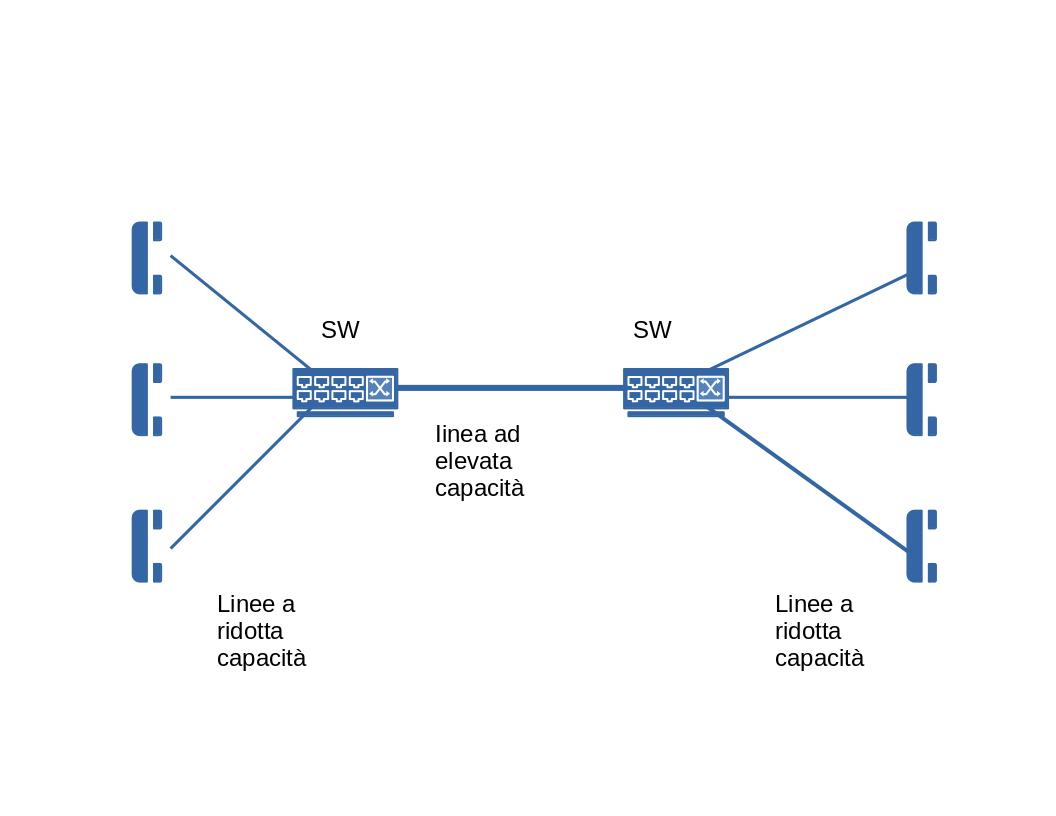
\includegraphics[weight=4cm,height=8cm]{img/Reti a commutazione di circuito.jpg}
  \caption{Reti a commutazione di circuito}
\end{figure}
\subsection{Reti a commutazione di pacchetto}
\begin{itemize}
\item Due dispositivi si scambiano blocchi di dati ({\tt pacchetto})
\item Lo {\it switch} può memorizzare i pacchetti per inviarli successivamente
\item più tipicamente funzione svolta dal {\em router}
\end{itemize}
\begin{figure}[!h]
  \centering
  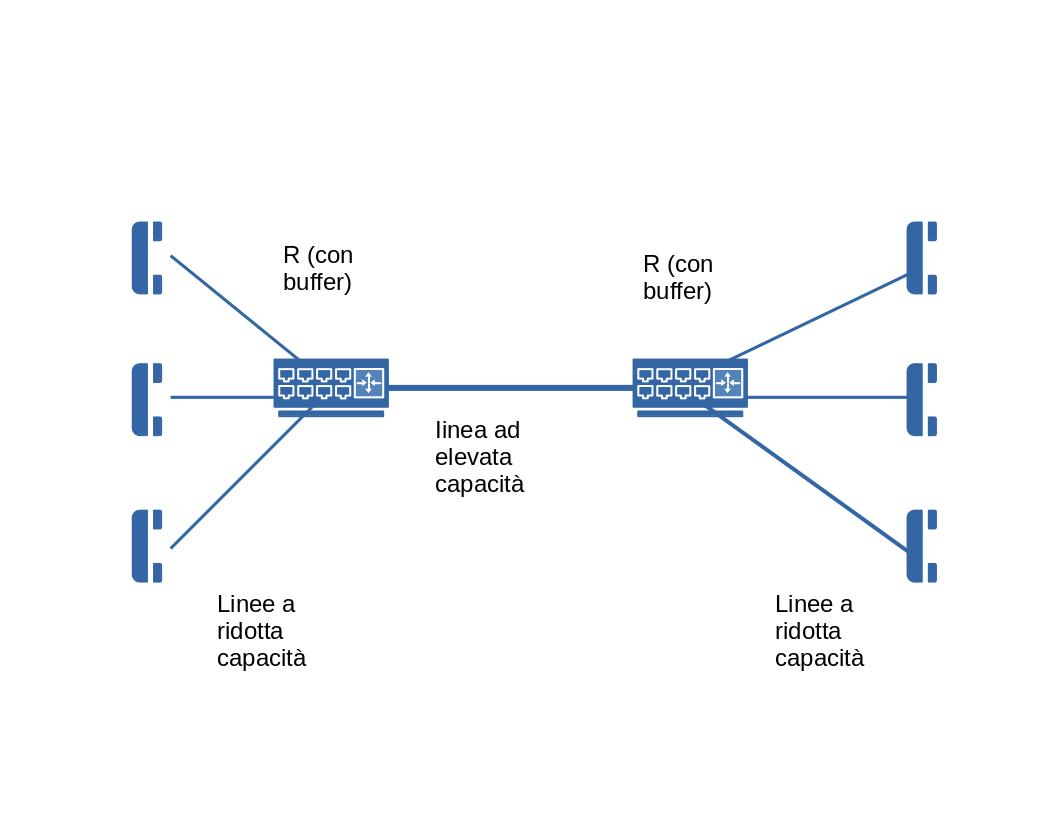
\includegraphics[weight=4cm,height=8cm]{img/Reti a commutazione di pacchetto.jpg}
  \caption{Reti a commutazione di pacchetto}
\end{figure}
\subsection{Implementazioni}
\begin{itemize}
\item Il sistema PDH non è univoco ovunque, me prevede tre standard differenti
  \begin{itemize}
  \item europeo (sistema analogo in india) con base a 32 canali
  \item statunitense con base a 24 canali
  \item giapponese con base a 24 canali
  \end{itemize}
\item Condividono lo stesso meccanismo di base ma differiscono per alcuni dettagli di funzionamento e per le gerarchie di multiplazione
  \begin{itemize}
  \item di fatto assenza di interoperabilità
  \item di fatto poco usati oggigiorno
    \begin{itemize}
    \item sostituiti da sistemi SDH ({\bf che vedremo più avanti in questa lezione})
    \item attivi solo nelle zone terminali delle reti per la multiplazione di traffico telefonico
    \end{itemize}
  \end{itemize}
\end{itemize}
\subsection{Canali telefonici digitali}
\begin{itemize}
\item Modulazione a impulsi codificati
  \begin{itemize}
  \item {\tt Pulse-Code Modulation (PCM)}
  \item anche in altre applicazioni come CD e DVD
  \end{itemize}
\item Campionamento + quantizzazione + rappresentazione binaria (ADC/DAC)
  \begin{itemize}
  \item quantizzazione operazione rumorosa
  \item 8, 16, 20 o 24 bit per campione
  \end{itemize}
\item PCM lineare: i livelli quantizzazione sono linearmente uniformi
\item PCM non lineare
  \begin{itemize}
  \item i segnali maggiormente affetti dell'approssimazione sono quelli a bassa intensità (errore relativo maggiore)
    \item quantizzazione non lineare: livelli più piccoli e ravvicinati nella regione di segnale debole e più distanziati nella regione in cui il segnale è più intenso
  \end{itemize}
\end{itemize}


\chapter{Applicazione delle reti}
\printindex
\end{document}
